\documentclass[1p]{elsarticle_modified}
%\bibliographystyle{elsarticle-num}

%\usepackage[colorlinks]{hyperref}
%\usepackage{abbrmath_seonhwa} %\Abb, \Ascr, \Acal ,\Abf, \Afrak
\usepackage{amsfonts}
\usepackage{amssymb}
\usepackage{amsmath}
\usepackage{amsthm}
\usepackage{scalefnt}
\usepackage{amsbsy}
\usepackage{kotex}
\usepackage{caption}
\usepackage{subfig}
\usepackage{color}
\usepackage{graphicx}
\usepackage{xcolor} %% white, black, red, green, blue, cyan, magenta, yellow
\usepackage{float}
\usepackage{setspace}
\usepackage{hyperref}

\usepackage{tikz}
\usetikzlibrary{arrows}

\usepackage{multirow}
\usepackage{array} % fixed length table
\usepackage{hhline}

%%%%%%%%%%%%%%%%%%%%%
\makeatletter
\renewcommand*\env@matrix[1][\arraystretch]{%
	\edef\arraystretch{#1}%
	\hskip -\arraycolsep
	\let\@ifnextchar\new@ifnextchar
	\array{*\c@MaxMatrixCols c}}
\makeatother %https://tex.stackexchange.com/questions/14071/how-can-i-increase-the-line-spacing-in-a-matrix
%%%%%%%%%%%%%%%

\usepackage[normalem]{ulem}

\newcommand{\msout}[1]{\ifmmode\text{\sout{\ensuremath{#1}}}\else\sout{#1}\fi}
%SOURCE: \msout is \stkout macro in https://tex.stackexchange.com/questions/20609/strikeout-in-math-mode

\newcommand{\cancel}[1]{
	\ifmmode
	{\color{red}\msout{#1}}
	\else
	{\color{red}\sout{#1}}
	\fi
}

\newcommand{\add}[1]{
	{\color{blue}\uwave{#1}}
}

\newcommand{\replace}[2]{
	\ifmmode
	{\color{red}\msout{#1}}{\color{blue}\uwave{#2}}
	\else
	{\color{red}\sout{#1}}{\color{blue}\uwave{#2}}
	\fi
}

\newcommand{\Sol}{\mathcal{S}} %segment
\newcommand{\D}{D} %diagram
\newcommand{\A}{\mathcal{A}} %arc


%%%%%%%%%%%%%%%%%%%%%%%%%%%%%5 test

\def\sl{\operatorname{\textup{SL}}(2,\Cbb)}
\def\psl{\operatorname{\textup{PSL}}(2,\Cbb)}
\def\quan{\mkern 1mu \triangleright \mkern 1mu}

\theoremstyle{definition}
\newtheorem{thm}{Theorem}[section]
\newtheorem{prop}[thm]{Proposition}
\newtheorem{lem}[thm]{Lemma}
\newtheorem{ques}[thm]{Question}
\newtheorem{cor}[thm]{Corollary}
\newtheorem{defn}[thm]{Definition}
\newtheorem{exam}[thm]{Example}
\newtheorem{rmk}[thm]{Remark}
\newtheorem{alg}[thm]{Algorithm}

\newcommand{\I}{\sqrt{-1}}
\begin{document}

%\begin{frontmatter}
%
%\title{Boundary parabolic representations of knots up to 8 crossings}
%
%%% Group authors per affiliation:
%\author{Yunhi Cho} 
%\address{Department of Mathematics, University of Seoul, Seoul, Korea}
%\ead{yhcho@uos.ac.kr}
%
%
%\author{Seonhwa Kim} %\fnref{s_kim}}
%\address{Center for Geometry and Physics, Institute for Basic Science, Pohang, 37673, Korea}
%\ead{ryeona17@ibs.re.kr}
%
%\author{Hyuk Kim}
%\address{Department of Mathematical Sciences, Seoul National University, Seoul 08826, Korea}
%\ead{hyukkim@snu.ac.kr}
%
%\author{Seokbeom Yoon}
%\address{Department of Mathematical Sciences, Seoul National University, Seoul, 08826,  Korea}
%\ead{sbyoon15@snu.ac.kr}
%
%\begin{abstract}
%We find all boundary parabolic representation of knots up to 8 crossings.
%
%\end{abstract}
%\begin{keyword}
%    \MSC[2010] 57M25 
%\end{keyword}
%
%\end{frontmatter}

%\linenumbers
%\tableofcontents
%
\newcommand\colored[1]{\textcolor{white}{\rule[-0.35ex]{0.8em}{1.4ex}}\kern-0.8em\color{red} #1}%
%\newcommand\colored[1]{\textcolor{white}{ #1}\kern-2.17ex	\textcolor{white}{ #1}\kern-1.81ex	\textcolor{white}{ #1}\kern-2.15ex\color{red}#1	}

{\Large $\underline{12a_{1061}~(K12a_{1061})}$}

\setlength{\tabcolsep}{10pt}
\renewcommand{\arraystretch}{1.6}
\vspace{1cm}\begin{tabular}{m{100pt}>{\centering\arraybackslash}m{274pt}}
\multirow{5}{120pt}{
	\centering
	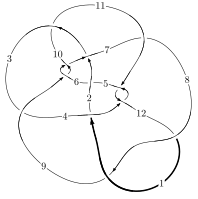
\includegraphics[width=112pt]{../../../GIT/diagram.site/Diagrams/png/1862_12a_1061.png}\\
\ \ \ A knot diagram\footnotemark}&
\allowdisplaybreaks
\textbf{Linearized knot diagam} \\
\cline{2-2}
 &
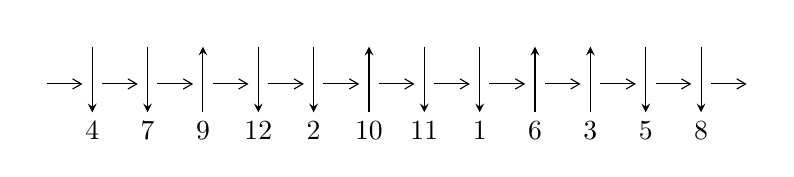
\begin{tikzpicture}[x=20pt, y=17pt]
	% nodes
	\node (C0) at (0, 0) {};
	\node (C1) at (1, 0) {};
	\node (C1U) at (1, +1) {};
	\node (C1D) at (1, -1) {4};

	\node (C2) at (2, 0) {};
	\node (C2U) at (2, +1) {};
	\node (C2D) at (2, -1) {7};

	\node (C3) at (3, 0) {};
	\node (C3U) at (3, +1) {};
	\node (C3D) at (3, -1) {9};

	\node (C4) at (4, 0) {};
	\node (C4U) at (4, +1) {};
	\node (C4D) at (4, -1) {12};

	\node (C5) at (5, 0) {};
	\node (C5U) at (5, +1) {};
	\node (C5D) at (5, -1) {2};

	\node (C6) at (6, 0) {};
	\node (C6U) at (6, +1) {};
	\node (C6D) at (6, -1) {10};

	\node (C7) at (7, 0) {};
	\node (C7U) at (7, +1) {};
	\node (C7D) at (7, -1) {11};

	\node (C8) at (8, 0) {};
	\node (C8U) at (8, +1) {};
	\node (C8D) at (8, -1) {1};

	\node (C9) at (9, 0) {};
	\node (C9U) at (9, +1) {};
	\node (C9D) at (9, -1) {6};

	\node (C10) at (10, 0) {};
	\node (C10U) at (10, +1) {};
	\node (C10D) at (10, -1) {3};

	\node (C11) at (11, 0) {};
	\node (C11U) at (11, +1) {};
	\node (C11D) at (11, -1) {5};

	\node (C12) at (12, 0) {};
	\node (C12U) at (12, +1) {};
	\node (C12D) at (12, -1) {8};
	\node (C13) at (13, 0) {};

	% arrows
	\draw[->,>={angle 60}]
	(C0) edge (C1) (C1) edge (C2) (C2) edge (C3) (C3) edge (C4) (C4) edge (C5) (C5) edge (C6) (C6) edge (C7) (C7) edge (C8) (C8) edge (C9) (C9) edge (C10) (C10) edge (C11) (C11) edge (C12) (C12) edge (C13) ;	\draw[->,>=stealth]
	(C1U) edge (C1D) (C2U) edge (C2D) (C3D) edge (C3U) (C4U) edge (C4D) (C5U) edge (C5D) (C6D) edge (C6U) (C7U) edge (C7D) (C8U) edge (C8D) (C9D) edge (C9U) (C10D) edge (C10U) (C11U) edge (C11D) (C12U) edge (C12D) ;
	\end{tikzpicture} \\
\hhline{~~} \\& 
\textbf{Solving Sequence} \\ \cline{2-2} 
 &
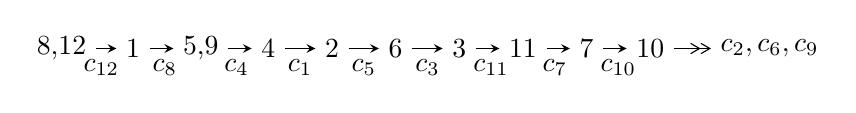
\begin{tikzpicture}[x=23pt, y=7pt]
	% node
	\node (A0) at (-1/8, 0) {8,12};
	\node (A1) at (1, 0) {1};
	\node (A2) at (33/16, 0) {5,9};
	\node (A3) at (25/8, 0) {4};
	\node (A4) at (33/8, 0) {2};
	\node (A5) at (41/8, 0) {6};
	\node (A6) at (49/8, 0) {3};
	\node (A7) at (57/8, 0) {11};
	\node (A8) at (65/8, 0) {7};
	\node (A9) at (73/8, 0) {10};
	\node (C1) at (1/2, -1) {$c_{12}$};
	\node (C2) at (3/2, -1) {$c_{8}$};
	\node (C3) at (21/8, -1) {$c_{4}$};
	\node (C4) at (29/8, -1) {$c_{1}$};
	\node (C5) at (37/8, -1) {$c_{5}$};
	\node (C6) at (45/8, -1) {$c_{3}$};
	\node (C7) at (53/8, -1) {$c_{11}$};
	\node (C8) at (61/8, -1) {$c_{7}$};
	\node (C9) at (69/8, -1) {$c_{10}$};
	\node (A10) at (11, 0) {$c_{2},c_{6},c_{9}$};

	% edge
	\draw[->,>=stealth]	
	(A0) edge (A1) (A1) edge (A2) (A2) edge (A3) (A3) edge (A4) (A4) edge (A5) (A5) edge (A6) (A6) edge (A7) (A7) edge (A8) (A8) edge (A9) ;
	\draw[->>,>={angle 60}]	
	(A9) edge (A10);
\end{tikzpicture} \\ 

\end{tabular} \\

\footnotetext{
The image of knot diagram is generated by the software ``\textbf{Draw programme}" developed by Andrew Bartholomew(\url{http://www.layer8.co.uk/maths/draw/index.htm\#Running-draw}), where we modified some parts for our purpose(\url{https://github.com/CATsTAILs/LinksPainter}).
}\phantom \\ \newline 
\centering \textbf{Ideals for irreducible components\footnotemark of $X_{\text{par}}$} 
 
\begin{align*}
I^u_{1}&=\langle 
-3.43650\times10^{1121} u^{176}+7.56229\times10^{1121} u^{175}+\cdots+7.16415\times10^{1120} b-1.78638\times10^{1125},\\
\phantom{I^u_{1}}&\phantom{= \langle  }1.87678\times10^{1125} u^{176}-4.17003\times10^{1125} u^{175}+\cdots+3.00966\times10^{1124} a+1.00424\times10^{1129},\\
\phantom{I^u_{1}}&\phantom{= \langle  }u^{177}-3 u^{176}+\cdots+99313 u-4201\rangle \\
I^u_{2}&=\langle 
1.31741\times10^{47} u^{40}-3.05294\times10^{47} u^{39}+\cdots+3.87165\times10^{46} b-2.49858\times10^{47},\\
\phantom{I^u_{2}}&\phantom{= \langle  }1.95215\times10^{46} u^{40}-6.23390\times10^{46} u^{39}+\cdots+3.87165\times10^{46} a-1.19738\times10^{47},\;u^{41}-3 u^{40}+\cdots-7 u+1\rangle \\
I^u_{3}&=\langle 
b-1,\;a,\;u+1\rangle \\
I^u_{4}&=\langle 
b+a+2,\;a^2+3 a+3,\;u+1\rangle \\
\\
\end{align*}
\raggedright * 4 irreducible components of $\dim_{\mathbb{C}}=0$, with total 221 representations.\\
\footnotetext{All coefficients of polynomials are rational numbers. But the coefficients are sometimes approximated in decimal forms when there is not enough margin.}
\newpage
\renewcommand{\arraystretch}{1}
\centering \section*{I. $I^u_{1}= \langle -3.44\times10^{1121} u^{176}+7.56\times10^{1121} u^{175}+\cdots+7.16\times10^{1120} b-1.79\times10^{1125},\;1.88\times10^{1125} u^{176}-4.17\times10^{1125} u^{175}+\cdots+3.01\times10^{1124} a+1.00\times10^{1129},\;u^{177}-3 u^{176}+\cdots+99313 u-4201 \rangle$}
\flushleft \textbf{(i) Arc colorings}\\
\begin{tabular}{m{7pt} m{180pt} m{7pt} m{180pt} }
\flushright $a_{8}=$&$\begin{pmatrix}0\\u\end{pmatrix}$ \\
\flushright $a_{12}=$&$\begin{pmatrix}1\\0\end{pmatrix}$ \\
\flushright $a_{1}=$&$\begin{pmatrix}1\\u^2\end{pmatrix}$ \\
\flushright $a_{5}=$&$\begin{pmatrix}-6.23586 u^{176}+13.8555 u^{175}+\cdots+746239. u-33367.2\\4.79679 u^{176}-10.5557 u^{175}+\cdots-558500. u+24935.0\end{pmatrix}$ \\
\flushright $a_{9}=$&$\begin{pmatrix}- u\\- u^3+u\end{pmatrix}$ \\
\flushright $a_{4}=$&$\begin{pmatrix}-1.43906 u^{176}+3.29974 u^{175}+\cdots+187738. u-8432.18\\4.79679 u^{176}-10.5557 u^{175}+\cdots-558500. u+24935.0\end{pmatrix}$ \\
\flushright $a_{2}=$&$\begin{pmatrix}7.39483 u^{176}-16.3425 u^{175}+\cdots-883940. u+39499.8\\5.95064 u^{176}-12.5957 u^{175}+\cdots-634341. u+28159.7\end{pmatrix}$ \\
\flushright $a_{6}=$&$\begin{pmatrix}-3.66260 u^{176}+7.48021 u^{175}+\cdots+351755. u-15523.3\\2.55481 u^{176}-5.37588 u^{175}+\cdots-263974. u+11698.7\end{pmatrix}$ \\
\flushright $a_{3}=$&$\begin{pmatrix}-4.07792 u^{176}+9.10767 u^{175}+\cdots+494085. u-22108.6\\5.74228 u^{176}-12.6241 u^{175}+\cdots-666518. u+29753.1\end{pmatrix}$ \\
\flushright $a_{11}=$&$\begin{pmatrix}4.74044 u^{176}-9.94666 u^{175}+\cdots-492414. u+21828.5\\-8.52570 u^{176}+18.2057 u^{175}+\cdots+925988. u-41169.2\end{pmatrix}$ \\
\flushright $a_{7}=$&$\begin{pmatrix}1.33544 u^{176}-2.95521 u^{175}+\cdots-152453. u+6810.67\\4.62485 u^{176}-9.86075 u^{175}+\cdots-502238. u+22311.0\end{pmatrix}$ \\
\flushright $a_{10}=$&$\begin{pmatrix}2.03076 u^{176}-3.92794 u^{175}+\cdots-167606. u+7302.95\\-4.32743 u^{176}+9.10927 u^{175}+\cdots+454536. u-20152.1\end{pmatrix}$\\&\end{tabular}
\flushleft \textbf{(ii) Obstruction class $= -1$}\\~\\
\flushleft \textbf{(iii) Cusp Shapes $= 0.576507 u^{176}-1.54492 u^{175}+\cdots-73177.9 u+3324.73$}\\~\\
\newpage\renewcommand{\arraystretch}{1}
\flushleft \textbf{(iv) u-Polynomials at the component}\newline \\
\begin{tabular}{m{50pt}|m{274pt}}
Crossings & \hspace{64pt}u-Polynomials at each crossing \\
\hline $$\begin{aligned}c_{1}\end{aligned}$$&$\begin{aligned}
&u^{177}+12 u^{176}+\cdots+594886 u-71806
\end{aligned}$\\
\hline $$\begin{aligned}c_{2}\end{aligned}$$&$\begin{aligned}
&u^{177}-2 u^{176}+\cdots-307 u+29
\end{aligned}$\\
\hline $$\begin{aligned}c_{3}\end{aligned}$$&$\begin{aligned}
&u^{177}- u^{176}+\cdots+20299788 u-41864904
\end{aligned}$\\
\hline $$\begin{aligned}c_{4},c_{11}\end{aligned}$$&$\begin{aligned}
&u^{177}+57 u^{175}+\cdots-3987 u-577
\end{aligned}$\\
\hline $$\begin{aligned}c_{5}\end{aligned}$$&$\begin{aligned}
&u^{177}-3 u^{176}+\cdots+571133 u+16391
\end{aligned}$\\
\hline $$\begin{aligned}c_{6},c_{9}\end{aligned}$$&$\begin{aligned}
&u^{177}+u^{176}+\cdots-4688 u-248
\end{aligned}$\\
\hline $$\begin{aligned}c_{7}\end{aligned}$$&$\begin{aligned}
&u^{177}+5 u^{176}+\cdots+575187597 u+140105457
\end{aligned}$\\
\hline $$\begin{aligned}c_{8},c_{12}\end{aligned}$$&$\begin{aligned}
&u^{177}-3 u^{176}+\cdots+99313 u-4201
\end{aligned}$\\
\hline $$\begin{aligned}c_{10}\end{aligned}$$&$\begin{aligned}
&u^{177}+3 u^{176}+\cdots-2447 u+211
\end{aligned}$\\
\hline
\end{tabular}\\~\\
\newpage\renewcommand{\arraystretch}{1}
\flushleft \textbf{(v) Riley Polynomials at the component}\newline \\
\begin{tabular}{m{50pt}|m{274pt}}
Crossings & \hspace{64pt}Riley Polynomials at each crossing \\
\hline $$\begin{aligned}c_{1}\end{aligned}$$&$\begin{aligned}
&y^{177}-24 y^{176}+\cdots+59480875472 y-5156101636
\end{aligned}$\\
\hline $$\begin{aligned}c_{2}\end{aligned}$$&$\begin{aligned}
&y^{177}+14 y^{176}+\cdots+22677 y-841
\end{aligned}$\\
\hline $$\begin{aligned}c_{3}\end{aligned}$$&$\begin{aligned}
&y^{177}+93 y^{176}+\cdots-69206595705210672 y-1752670186929216
\end{aligned}$\\
\hline $$\begin{aligned}c_{4},c_{11}\end{aligned}$$&$\begin{aligned}
&y^{177}+114 y^{176}+\cdots-9098317 y-332929
\end{aligned}$\\
\hline $$\begin{aligned}c_{5}\end{aligned}$$&$\begin{aligned}
&y^{177}+5 y^{176}+\cdots-252864312125 y-268664881
\end{aligned}$\\
\hline $$\begin{aligned}c_{6},c_{9}\end{aligned}$$&$\begin{aligned}
&y^{177}-107 y^{176}+\cdots+3350560 y-61504
\end{aligned}$\\
\hline $$\begin{aligned}c_{7}\end{aligned}$$&$\begin{aligned}
&y^{177}-71 y^{176}+\cdots+1502416853582876793 y-19629539081178849
\end{aligned}$\\
\hline $$\begin{aligned}c_{8},c_{12}\end{aligned}$$&$\begin{aligned}
&y^{177}-109 y^{176}+\cdots+3935864265 y-17648401
\end{aligned}$\\
\hline $$\begin{aligned}c_{10}\end{aligned}$$&$\begin{aligned}
&y^{177}+13 y^{176}+\cdots+3237213 y-44521
\end{aligned}$\\
\hline
\end{tabular}\\~\\
\newpage\flushleft \textbf{(vi) Complex Volumes and Cusp Shapes}
$$\begin{array}{c|c|c}  
\text{Solutions to }I^u_{1}& \I (\text{vol} + \sqrt{-1}CS) & \text{Cusp shape}\\
 \hline 
\begin{aligned}
u &= \phantom{-}0.391552 + 0.918289 I \\
a &= -0.02443 - 1.43307 I \\
b &= \phantom{-}0.311790 + 1.248170 I\end{aligned}
 & \phantom{-}3.99925 - 5.25642 I & \phantom{-0.000000 } 0 \\ \hline\begin{aligned}
u &= \phantom{-}0.391552 - 0.918289 I \\
a &= -0.02443 + 1.43307 I \\
b &= \phantom{-}0.311790 - 1.248170 I\end{aligned}
 & \phantom{-}3.99925 + 5.25642 I & \phantom{-0.000000 } 0 \\ \hline\begin{aligned}
u &= -1.012290 + 0.102932 I \\
a &= \phantom{-}1.28657 + 2.53369 I \\
b &= \phantom{-}0.283305 - 1.151170 I\end{aligned}
 & -2.77341 + 4.32190 I & \phantom{-0.000000 } 0 \\ \hline\begin{aligned}
u &= -1.012290 - 0.102932 I \\
a &= \phantom{-}1.28657 - 2.53369 I \\
b &= \phantom{-}0.283305 + 1.151170 I\end{aligned}
 & -2.77341 - 4.32190 I & \phantom{-0.000000 } 0 \\ \hline\begin{aligned}
u &= -1.005330 + 0.205847 I \\
a &= \phantom{-}0.594212 + 0.562437 I \\
b &= \phantom{-}1.15485 - 1.02978 I\end{aligned}
 & -2.46905 + 1.67974 I & \phantom{-0.000000 } 0 \\ \hline\begin{aligned}
u &= -1.005330 - 0.205847 I \\
a &= \phantom{-}0.594212 - 0.562437 I \\
b &= \phantom{-}1.15485 + 1.02978 I\end{aligned}
 & -2.46905 - 1.67974 I & \phantom{-0.000000 } 0 \\ \hline\begin{aligned}
u &= -0.357186 + 0.902669 I \\
a &= \phantom{-}0.01351 + 1.56060 I \\
b &= -0.097222 - 1.287070 I\end{aligned}
 & \phantom{-}9.03240 + 3.28339 I & \phantom{-0.000000 } 0 \\ \hline\begin{aligned}
u &= -0.357186 - 0.902669 I \\
a &= \phantom{-}0.01351 - 1.56060 I \\
b &= -0.097222 + 1.287070 I\end{aligned}
 & \phantom{-}9.03240 - 3.28339 I & \phantom{-0.000000 } 0 \\ \hline\begin{aligned}
u &= \phantom{-}1.009020 + 0.221811 I \\
a &= -1.002600 - 0.124917 I \\
b &= -0.491454 - 1.138300 I\end{aligned}
 & \phantom{-}4.31608 - 4.96383 I & \phantom{-0.000000 } 0 \\ \hline\begin{aligned}
u &= \phantom{-}1.009020 - 0.221811 I \\
a &= -1.002600 + 0.124917 I \\
b &= -0.491454 + 1.138300 I\end{aligned}
 & \phantom{-}4.31608 + 4.96383 I & \phantom{-0.000000 } 0\\
 \hline 
 \end{array}$$\newpage$$\begin{array}{c|c|c}  
\text{Solutions to }I^u_{1}& \I (\text{vol} + \sqrt{-1}CS) & \text{Cusp shape}\\
 \hline 
\begin{aligned}
u &= \phantom{-}0.954921 + 0.131917 I \\
a &= -0.165525 + 0.847085 I \\
b &= \phantom{-}0.15331 - 1.99846 I\end{aligned}
 & \phantom{-}3.09098 - 7.15631 I & \phantom{-0.000000 } 0 \\ \hline\begin{aligned}
u &= \phantom{-}0.954921 - 0.131917 I \\
a &= -0.165525 - 0.847085 I \\
b &= \phantom{-}0.15331 + 1.99846 I\end{aligned}
 & \phantom{-}3.09098 + 7.15631 I & \phantom{-0.000000 } 0 \\ \hline\begin{aligned}
u &= -0.601828 + 0.848506 I \\
a &= -0.474569 - 0.879284 I \\
b &= \phantom{-}0.546943 + 1.187910 I\end{aligned}
 & \phantom{-}5.13827 - 6.39341 I & \phantom{-0.000000 } 0 \\ \hline\begin{aligned}
u &= -0.601828 - 0.848506 I \\
a &= -0.474569 + 0.879284 I \\
b &= \phantom{-}0.546943 - 1.187910 I\end{aligned}
 & \phantom{-}5.13827 + 6.39341 I & \phantom{-0.000000 } 0 \\ \hline\begin{aligned}
u &= -0.940544 + 0.156825 I \\
a &= -0.841523 - 0.353184 I \\
b &= \phantom{-}0.10065 + 2.46271 I\end{aligned}
 & -0.014440 + 0.601529 I & \phantom{-0.000000 } 0 \\ \hline\begin{aligned}
u &= -0.940544 - 0.156825 I \\
a &= -0.841523 + 0.353184 I \\
b &= \phantom{-}0.10065 - 2.46271 I\end{aligned}
 & -0.014440 - 0.601529 I & \phantom{-0.000000 } 0 \\ \hline\begin{aligned}
u &= -1.047200 + 0.040846 I \\
a &= -1.32597 + 0.71142 I \\
b &= -0.583943 - 0.997112 I\end{aligned}
 & -2.69528 - 1.02232 I & \phantom{-0.000000 } 0 \\ \hline\begin{aligned}
u &= -1.047200 - 0.040846 I \\
a &= -1.32597 - 0.71142 I \\
b &= -0.583943 + 0.997112 I\end{aligned}
 & -2.69528 + 1.02232 I & \phantom{-0.000000 } 0 \\ \hline\begin{aligned}
u &= -0.947260 + 0.087408 I \\
a &= -0.657882 - 1.027030 I \\
b &= -0.17504 + 1.71746 I\end{aligned}
 & -0.310754 + 0.951044 I & \phantom{-0.000000 } 0 \\ \hline\begin{aligned}
u &= -0.947260 - 0.087408 I \\
a &= -0.657882 + 1.027030 I \\
b &= -0.17504 - 1.71746 I\end{aligned}
 & -0.310754 - 0.951044 I & \phantom{-0.000000 } 0\\
 \hline 
 \end{array}$$\newpage$$\begin{array}{c|c|c}  
\text{Solutions to }I^u_{1}& \I (\text{vol} + \sqrt{-1}CS) & \text{Cusp shape}\\
 \hline 
\begin{aligned}
u &= \phantom{-}0.946237 + 0.090615 I \\
a &= -1.61285 - 0.57839 I \\
b &= -0.647048 + 0.811473 I\end{aligned}
 & -2.16420 - 1.16727 I & \phantom{-0.000000 } 0 \\ \hline\begin{aligned}
u &= \phantom{-}0.946237 - 0.090615 I \\
a &= -1.61285 + 0.57839 I \\
b &= -0.647048 - 0.811473 I\end{aligned}
 & -2.16420 + 1.16727 I & \phantom{-0.000000 } 0 \\ \hline\begin{aligned}
u &= \phantom{-}0.945673 + 0.457721 I \\
a &= -1.58538 + 1.27224 I \\
b &= -0.102125 - 0.727054 I\end{aligned}
 & -2.33271 - 1.50229 I & \phantom{-0.000000 } 0 \\ \hline\begin{aligned}
u &= \phantom{-}0.945673 - 0.457721 I \\
a &= -1.58538 - 1.27224 I \\
b &= -0.102125 + 0.727054 I\end{aligned}
 & -2.33271 + 1.50229 I & \phantom{-0.000000 } 0 \\ \hline\begin{aligned}
u &= -0.915295 + 0.098878 I \\
a &= -1.168990 - 0.165690 I \\
b &= -0.314651 + 1.249200 I\end{aligned}
 & -0.273272 + 0.052849 I & \phantom{-0.000000 } 0 \\ \hline\begin{aligned}
u &= -0.915295 - 0.098878 I \\
a &= -1.168990 + 0.165690 I \\
b &= -0.314651 - 1.249200 I\end{aligned}
 & -0.273272 - 0.052849 I & \phantom{-0.000000 } 0 \\ \hline\begin{aligned}
u &= -0.353857 + 1.019980 I \\
a &= -0.18650 - 1.57502 I \\
b &= \phantom{-}0.319256 + 0.686065 I\end{aligned}
 & -0.221550 - 1.267490 I & \phantom{-0.000000 } 0 \\ \hline\begin{aligned}
u &= -0.353857 - 1.019980 I \\
a &= -0.18650 + 1.57502 I \\
b &= \phantom{-}0.319256 - 0.686065 I\end{aligned}
 & -0.221550 + 1.267490 I & \phantom{-0.000000 } 0 \\ \hline\begin{aligned}
u &= \phantom{-}0.531566 + 0.747089 I \\
a &= \phantom{-}0.87660 - 1.28314 I \\
b &= -0.123206 + 1.042790 I\end{aligned}
 & \phantom{-}3.34181 + 0.08527 I & \phantom{-0.000000 } 0 \\ \hline\begin{aligned}
u &= \phantom{-}0.531566 - 0.747089 I \\
a &= \phantom{-}0.87660 + 1.28314 I \\
b &= -0.123206 - 1.042790 I\end{aligned}
 & \phantom{-}3.34181 - 0.08527 I & \phantom{-0.000000 } 0\\
 \hline 
 \end{array}$$\newpage$$\begin{array}{c|c|c}  
\text{Solutions to }I^u_{1}& \I (\text{vol} + \sqrt{-1}CS) & \text{Cusp shape}\\
 \hline 
\begin{aligned}
u &= -1.09324\phantom{ +0.000000I} \\
a &= \phantom{-}0.220975\phantom{ +0.000000I} \\
b &= \phantom{-}0.820855\phantom{ +0.000000I}\end{aligned}
 & -2.10948\phantom{ +0.000000I} & \phantom{-0.000000 } 0 \\ \hline\begin{aligned}
u &= \phantom{-}1.086460 + 0.145851 I \\
a &= -1.44175 + 1.27828 I \\
b &= -0.368075 - 0.833229 I\end{aligned}
 & -3.80034 - 1.23674 I & \phantom{-0.000000 } 0 \\ \hline\begin{aligned}
u &= \phantom{-}1.086460 - 0.145851 I \\
a &= -1.44175 - 1.27828 I \\
b &= -0.368075 + 0.833229 I\end{aligned}
 & -3.80034 + 1.23674 I & \phantom{-0.000000 } 0 \\ \hline\begin{aligned}
u &= -0.908512 + 0.619518 I \\
a &= \phantom{-}0.51159 + 1.40686 I \\
b &= \phantom{-}0.472021 - 1.307320 I\end{aligned}
 & \phantom{-}2.51715 + 5.30103 I & \phantom{-0.000000 } 0 \\ \hline\begin{aligned}
u &= -0.908512 - 0.619518 I \\
a &= \phantom{-}0.51159 - 1.40686 I \\
b &= \phantom{-}0.472021 + 1.307320 I\end{aligned}
 & \phantom{-}2.51715 - 5.30103 I & \phantom{-0.000000 } 0 \\ \hline\begin{aligned}
u &= \phantom{-}0.734045 + 0.520091 I \\
a &= \phantom{-}0.900884 - 0.967272 I \\
b &= \phantom{-}0.831074 + 0.426101 I\end{aligned}
 & \phantom{-}2.50002 + 1.14829 I & \phantom{-0.000000 } 0 \\ \hline\begin{aligned}
u &= \phantom{-}0.734045 - 0.520091 I \\
a &= \phantom{-}0.900884 + 0.967272 I \\
b &= \phantom{-}0.831074 - 0.426101 I\end{aligned}
 & \phantom{-}2.50002 - 1.14829 I & \phantom{-0.000000 } 0 \\ \hline\begin{aligned}
u &= \phantom{-}1.094880 + 0.127112 I \\
a &= \phantom{-}1.64009 - 1.96992 I \\
b &= \phantom{-}0.363366 + 1.097080 I\end{aligned}
 & -0.84195 - 9.84986 I & \phantom{-0.000000 } 0 \\ \hline\begin{aligned}
u &= \phantom{-}1.094880 - 0.127112 I \\
a &= \phantom{-}1.64009 + 1.96992 I \\
b &= \phantom{-}0.363366 - 1.097080 I\end{aligned}
 & -0.84195 + 9.84986 I & \phantom{-0.000000 } 0 \\ \hline\begin{aligned}
u &= \phantom{-}0.376374 + 0.794396 I \\
a &= \phantom{-}0.42046 - 1.90181 I \\
b &= -0.246271 + 1.212780 I\end{aligned}
 & \phantom{-}3.77458 + 0.22570 I & \phantom{-0.000000 } 0\\
 \hline 
 \end{array}$$\newpage$$\begin{array}{c|c|c}  
\text{Solutions to }I^u_{1}& \I (\text{vol} + \sqrt{-1}CS) & \text{Cusp shape}\\
 \hline 
\begin{aligned}
u &= \phantom{-}0.376374 - 0.794396 I \\
a &= \phantom{-}0.42046 + 1.90181 I \\
b &= -0.246271 - 1.212780 I\end{aligned}
 & \phantom{-}3.77458 - 0.22570 I & \phantom{-0.000000 } 0 \\ \hline\begin{aligned}
u &= \phantom{-}0.757057 + 0.439147 I \\
a &= -0.303022 - 0.744920 I \\
b &= -0.021061 + 0.962905 I\end{aligned}
 & \phantom{-}2.31246 - 4.69016 I & \phantom{-0.000000 } 0 \\ \hline\begin{aligned}
u &= \phantom{-}0.757057 - 0.439147 I \\
a &= -0.303022 + 0.744920 I \\
b &= -0.021061 - 0.962905 I\end{aligned}
 & \phantom{-}2.31246 + 4.69016 I & \phantom{-0.000000 } 0 \\ \hline\begin{aligned}
u &= -0.301218 + 0.821230 I \\
a &= \phantom{-}0.798874 + 0.911540 I \\
b &= -0.668001 - 0.228977 I\end{aligned}
 & -3.41573 + 3.86998 I & \phantom{-0.000000 } 0 \\ \hline\begin{aligned}
u &= -0.301218 - 0.821230 I \\
a &= \phantom{-}0.798874 - 0.911540 I \\
b &= -0.668001 + 0.228977 I\end{aligned}
 & -3.41573 - 3.86998 I & \phantom{-0.000000 } 0 \\ \hline\begin{aligned}
u &= \phantom{-}1.062430 + 0.374783 I \\
a &= -1.018740 + 0.955399 I \\
b &= -0.83890 - 1.26580 I\end{aligned}
 & -0.99687 - 7.87321 I & \phantom{-0.000000 } 0 \\ \hline\begin{aligned}
u &= \phantom{-}1.062430 - 0.374783 I \\
a &= -1.018740 - 0.955399 I \\
b &= -0.83890 + 1.26580 I\end{aligned}
 & -0.99687 + 7.87321 I & \phantom{-0.000000 } 0 \\ \hline\begin{aligned}
u &= -1.128480 + 0.004016 I \\
a &= -1.24252 - 1.11842 I \\
b &= -0.347344 + 0.876242 I\end{aligned}
 & -3.05337 - 2.03135 I & \phantom{-0.000000 } 0 \\ \hline\begin{aligned}
u &= -1.128480 - 0.004016 I \\
a &= -1.24252 + 1.11842 I \\
b &= -0.347344 - 0.876242 I\end{aligned}
 & -3.05337 + 2.03135 I & \phantom{-0.000000 } 0 \\ \hline\begin{aligned}
u &= \phantom{-}0.855379\phantom{ +0.000000I} \\
a &= -0.0787454\phantom{ +0.000000I} \\
b &= \phantom{-}1.05081\phantom{ +0.000000I}\end{aligned}
 & -1.76038\phantom{ +0.000000I} & \phantom{-0.000000 } 0\\
 \hline 
 \end{array}$$\newpage$$\begin{array}{c|c|c}  
\text{Solutions to }I^u_{1}& \I (\text{vol} + \sqrt{-1}CS) & \text{Cusp shape}\\
 \hline 
\begin{aligned}
u &= -0.528790 + 1.018590 I \\
a &= \phantom{-}0.675767 + 1.062200 I \\
b &= -0.125160 - 1.163730 I\end{aligned}
 & \phantom{-}3.75788 + 0.64628 I & \phantom{-0.000000 } 0 \\ \hline\begin{aligned}
u &= -0.528790 - 1.018590 I \\
a &= \phantom{-}0.675767 - 1.062200 I \\
b &= -0.125160 + 1.163730 I\end{aligned}
 & \phantom{-}3.75788 - 0.64628 I & \phantom{-0.000000 } 0 \\ \hline\begin{aligned}
u &= \phantom{-}0.246315 + 1.127760 I \\
a &= -0.231005 + 1.156490 I \\
b &= \phantom{-}0.478466 - 1.045810 I\end{aligned}
 & \phantom{-}1.36757 + 5.18436 I & \phantom{-0.000000 } 0 \\ \hline\begin{aligned}
u &= \phantom{-}0.246315 - 1.127760 I \\
a &= -0.231005 - 1.156490 I \\
b &= \phantom{-}0.478466 + 1.045810 I\end{aligned}
 & \phantom{-}1.36757 - 5.18436 I & \phantom{-0.000000 } 0 \\ \hline\begin{aligned}
u &= -1.002010 + 0.588485 I \\
a &= -0.95049 - 1.14708 I \\
b &= -0.82139 + 1.16510 I\end{aligned}
 & \phantom{-}3.83121 + 11.73540 I & \phantom{-0.000000 } 0 \\ \hline\begin{aligned}
u &= -1.002010 - 0.588485 I \\
a &= -0.95049 + 1.14708 I \\
b &= -0.82139 - 1.16510 I\end{aligned}
 & \phantom{-}3.83121 - 11.73540 I & \phantom{-0.000000 } 0 \\ \hline\begin{aligned}
u &= \phantom{-}0.836072 + 0.055491 I \\
a &= \phantom{-}0.06630 + 1.54620 I \\
b &= \phantom{-}0.26188 - 1.54214 I\end{aligned}
 & \phantom{-}5.30380 + 3.62693 I & \phantom{-0.000000 } 0 \\ \hline\begin{aligned}
u &= \phantom{-}0.836072 - 0.055491 I \\
a &= \phantom{-}0.06630 - 1.54620 I \\
b &= \phantom{-}0.26188 + 1.54214 I\end{aligned}
 & \phantom{-}5.30380 - 3.62693 I & \phantom{-0.000000 } 0 \\ \hline\begin{aligned}
u &= \phantom{-}0.236989 + 0.801613 I \\
a &= \phantom{-}0.679542 - 0.281396 I \\
b &= -0.737005 + 0.266318 I\end{aligned}
 & \phantom{-}1.15113 + 3.41241 I & \phantom{-0.000000 } 0 \\ \hline\begin{aligned}
u &= \phantom{-}0.236989 - 0.801613 I \\
a &= \phantom{-}0.679542 + 0.281396 I \\
b &= -0.737005 - 0.266318 I\end{aligned}
 & \phantom{-}1.15113 - 3.41241 I & \phantom{-0.000000 } 0\\
 \hline 
 \end{array}$$\newpage$$\begin{array}{c|c|c}  
\text{Solutions to }I^u_{1}& \I (\text{vol} + \sqrt{-1}CS) & \text{Cusp shape}\\
 \hline 
\begin{aligned}
u &= \phantom{-}1.084080 + 0.447020 I \\
a &= \phantom{-}0.97770 - 1.26705 I \\
b &= \phantom{-}0.458533 + 1.204500 I\end{aligned}
 & \phantom{-}1.43428 - 4.53147 I & \phantom{-0.000000 } 0 \\ \hline\begin{aligned}
u &= \phantom{-}1.084080 - 0.447020 I \\
a &= \phantom{-}0.97770 + 1.26705 I \\
b &= \phantom{-}0.458533 - 1.204500 I\end{aligned}
 & \phantom{-}1.43428 + 4.53147 I & \phantom{-0.000000 } 0 \\ \hline\begin{aligned}
u &= -0.823083 + 0.082071 I \\
a &= \phantom{-}2.46000 - 0.71621 I \\
b &= -0.097261 - 0.714128 I\end{aligned}
 & -2.17701 - 3.32276 I & \phantom{-0.000000 } 0 \\ \hline\begin{aligned}
u &= -0.823083 - 0.082071 I \\
a &= \phantom{-}2.46000 + 0.71621 I \\
b &= -0.097261 + 0.714128 I\end{aligned}
 & -2.17701 + 3.32276 I & \phantom{-0.000000 } 0 \\ \hline\begin{aligned}
u &= \phantom{-}0.619532 + 0.532278 I \\
a &= \phantom{-}1.40729 - 1.05444 I \\
b &= -0.103957 + 0.860539 I\end{aligned}
 & \phantom{-}3.26068 + 0.10586 I & \phantom{-0.000000 } 0 \\ \hline\begin{aligned}
u &= \phantom{-}0.619532 - 0.532278 I \\
a &= \phantom{-}1.40729 + 1.05444 I \\
b &= -0.103957 - 0.860539 I\end{aligned}
 & \phantom{-}3.26068 - 0.10586 I & \phantom{-0.000000 } 0 \\ \hline\begin{aligned}
u &= \phantom{-}0.235191 + 0.767589 I \\
a &= \phantom{-}0.663443 - 1.134910 I \\
b &= -0.672235 + 0.108136 I\end{aligned}
 & \phantom{-}0.22989 - 9.90375 I & \phantom{-0.000000 } 0 \\ \hline\begin{aligned}
u &= \phantom{-}0.235191 - 0.767589 I \\
a &= \phantom{-}0.663443 + 1.134910 I \\
b &= -0.672235 - 0.108136 I\end{aligned}
 & \phantom{-}0.22989 + 9.90375 I & \phantom{-0.000000 } 0 \\ \hline\begin{aligned}
u &= -0.094807 + 1.196770 I \\
a &= \phantom{-}0.54562 - 1.40762 I \\
b &= -0.270772 + 1.077630 I\end{aligned}
 & \phantom{-}5.17093 + 1.54430 I & \phantom{-0.000000 } 0 \\ \hline\begin{aligned}
u &= -0.094807 - 1.196770 I \\
a &= \phantom{-}0.54562 + 1.40762 I \\
b &= -0.270772 - 1.077630 I\end{aligned}
 & \phantom{-}5.17093 - 1.54430 I & \phantom{-0.000000 } 0\\
 \hline 
 \end{array}$$\newpage$$\begin{array}{c|c|c}  
\text{Solutions to }I^u_{1}& \I (\text{vol} + \sqrt{-1}CS) & \text{Cusp shape}\\
 \hline 
\begin{aligned}
u &= \phantom{-}0.758171 + 0.196350 I \\
a &= -1.001890 - 0.051419 I \\
b &= -0.52968 - 1.33624 I\end{aligned}
 & \phantom{-}3.43079 + 5.49485 I & \phantom{-0.000000 } 0 \\ \hline\begin{aligned}
u &= \phantom{-}0.758171 - 0.196350 I \\
a &= -1.001890 + 0.051419 I \\
b &= -0.52968 + 1.33624 I\end{aligned}
 & \phantom{-}3.43079 - 5.49485 I & \phantom{-0.000000 } 0 \\ \hline\begin{aligned}
u &= -0.139158 + 1.211960 I \\
a &= \phantom{-}0.39126 + 1.50443 I \\
b &= -0.501028 - 1.155610 I\end{aligned}
 & -0.69121 - 8.40329 I & \phantom{-0.000000 } 0 \\ \hline\begin{aligned}
u &= -0.139158 - 1.211960 I \\
a &= \phantom{-}0.39126 - 1.50443 I \\
b &= -0.501028 + 1.155610 I\end{aligned}
 & -0.69121 + 8.40329 I & \phantom{-0.000000 } 0 \\ \hline\begin{aligned}
u &= -1.211060 + 0.170569 I \\
a &= -0.242241 + 0.041438 I \\
b &= -1.40337 - 0.27601 I\end{aligned}
 & -5.49092 + 1.00302 I & \phantom{-0.000000 } 0 \\ \hline\begin{aligned}
u &= -1.211060 - 0.170569 I \\
a &= -0.242241 - 0.041438 I \\
b &= -1.40337 + 0.27601 I\end{aligned}
 & -5.49092 - 1.00302 I & \phantom{-0.000000 } 0 \\ \hline\begin{aligned}
u &= \phantom{-}0.775060 + 0.053357 I \\
a &= \phantom{-}2.95172 - 0.60530 I \\
b &= -0.044043 - 0.639776 I\end{aligned}
 & \phantom{-}0.61289 - 9.15609 I & \phantom{-0.000000 } 0 \\ \hline\begin{aligned}
u &= \phantom{-}0.775060 - 0.053357 I \\
a &= \phantom{-}2.95172 + 0.60530 I \\
b &= -0.044043 + 0.639776 I\end{aligned}
 & \phantom{-}0.61289 + 9.15609 I & \phantom{-0.000000 } 0 \\ \hline\begin{aligned}
u &= \phantom{-}1.145010 + 0.455939 I \\
a &= \phantom{-}1.37527 - 1.22765 I \\
b &= \phantom{-}0.392644 + 1.231740 I\end{aligned}
 & \phantom{-}1.30786 - 4.87319 I & \phantom{-0.000000 } 0 \\ \hline\begin{aligned}
u &= \phantom{-}1.145010 - 0.455939 I \\
a &= \phantom{-}1.37527 + 1.22765 I \\
b &= \phantom{-}0.392644 - 1.231740 I\end{aligned}
 & \phantom{-}1.30786 + 4.87319 I & \phantom{-0.000000 } 0\\
 \hline 
 \end{array}$$\newpage$$\begin{array}{c|c|c}  
\text{Solutions to }I^u_{1}& \I (\text{vol} + \sqrt{-1}CS) & \text{Cusp shape}\\
 \hline 
\begin{aligned}
u &= -0.274998 + 0.714815 I \\
a &= -0.24924 + 2.24897 I \\
b &= -0.229992 - 1.328320 I\end{aligned}
 & \phantom{-}6.25952 - 6.72620 I & \phantom{-0.000000 } 0 \\ \hline\begin{aligned}
u &= -0.274998 - 0.714815 I \\
a &= -0.24924 - 2.24897 I \\
b &= -0.229992 + 1.328320 I\end{aligned}
 & \phantom{-}6.25952 + 6.72620 I & \phantom{-0.000000 } 0 \\ \hline\begin{aligned}
u &= -1.225960 + 0.288342 I \\
a &= -0.192662 - 0.093947 I \\
b &= \phantom{-}1.166860 + 0.459301 I\end{aligned}
 & -1.56928 + 1.41784 I & \phantom{-0.000000 } 0 \\ \hline\begin{aligned}
u &= -1.225960 - 0.288342 I \\
a &= -0.192662 + 0.093947 I \\
b &= \phantom{-}1.166860 - 0.459301 I\end{aligned}
 & -1.56928 - 1.41784 I & \phantom{-0.000000 } 0 \\ \hline\begin{aligned}
u &= -1.187910 + 0.424934 I \\
a &= \phantom{-}1.68999 + 0.79683 I \\
b &= \phantom{-}0.336471 - 1.178650 I\end{aligned}
 & \phantom{-}3.39460 + 11.05100 I & \phantom{-0.000000 } 0 \\ \hline\begin{aligned}
u &= -1.187910 - 0.424934 I \\
a &= \phantom{-}1.68999 - 0.79683 I \\
b &= \phantom{-}0.336471 + 1.178650 I\end{aligned}
 & \phantom{-}3.39460 - 11.05100 I & \phantom{-0.000000 } 0 \\ \hline\begin{aligned}
u &= \phantom{-}0.182314 + 0.714742 I \\
a &= -0.58197 + 1.32586 I \\
b &= \phantom{-}0.447162 - 1.173780 I\end{aligned}
 & \phantom{-}1.59912 + 4.11982 I & \phantom{-0.000000 } 0 \\ \hline\begin{aligned}
u &= \phantom{-}0.182314 - 0.714742 I \\
a &= -0.58197 - 1.32586 I \\
b &= \phantom{-}0.447162 + 1.173780 I\end{aligned}
 & \phantom{-}1.59912 - 4.11982 I & \phantom{-0.000000 } 0 \\ \hline\begin{aligned}
u &= \phantom{-}1.232390 + 0.278106 I \\
a &= \phantom{-}0.410103 - 0.833928 I \\
b &= \phantom{-}0.70988 + 1.33585 I\end{aligned}
 & \phantom{-}0.29249 - 6.31462 I & \phantom{-0.000000 } 0 \\ \hline\begin{aligned}
u &= \phantom{-}1.232390 - 0.278106 I \\
a &= \phantom{-}0.410103 + 0.833928 I \\
b &= \phantom{-}0.70988 - 1.33585 I\end{aligned}
 & \phantom{-}0.29249 + 6.31462 I & \phantom{-0.000000 } 0\\
 \hline 
 \end{array}$$\newpage$$\begin{array}{c|c|c}  
\text{Solutions to }I^u_{1}& \I (\text{vol} + \sqrt{-1}CS) & \text{Cusp shape}\\
 \hline 
\begin{aligned}
u &= \phantom{-}1.098370 + 0.627505 I \\
a &= -0.66043 + 1.76322 I \\
b &= -0.347388 - 1.026310 I\end{aligned}
 & -2.97291 - 2.92847 I & \phantom{-0.000000 } 0 \\ \hline\begin{aligned}
u &= \phantom{-}1.098370 - 0.627505 I \\
a &= -0.66043 - 1.76322 I \\
b &= -0.347388 + 1.026310 I\end{aligned}
 & -2.97291 + 2.92847 I & \phantom{-0.000000 } 0 \\ \hline\begin{aligned}
u &= -0.124925 + 0.722095 I \\
a &= \phantom{-}0.70437 + 1.70376 I \\
b &= \phantom{-}0.572944 - 0.399539 I\end{aligned}
 & -0.517939 - 0.978819 I & \phantom{-0.000000 } 0 \\ \hline\begin{aligned}
u &= -0.124925 - 0.722095 I \\
a &= \phantom{-}0.70437 - 1.70376 I \\
b &= \phantom{-}0.572944 + 0.399539 I\end{aligned}
 & -0.517939 + 0.978819 I & \phantom{-0.000000 } 0 \\ \hline\begin{aligned}
u &= \phantom{-}0.543119 + 0.490315 I \\
a &= \phantom{-}0.246827 + 0.177103 I \\
b &= -0.702628 + 0.738329 I\end{aligned}
 & \phantom{-}2.87974 - 5.20445 I & \phantom{-0.000000 } 0 \\ \hline\begin{aligned}
u &= \phantom{-}0.543119 - 0.490315 I \\
a &= \phantom{-}0.246827 - 0.177103 I \\
b &= -0.702628 - 0.738329 I\end{aligned}
 & \phantom{-}2.87974 + 5.20445 I & \phantom{-0.000000 } 0 \\ \hline\begin{aligned}
u &= -1.152640 + 0.540968 I \\
a &= \phantom{-}1.137750 + 0.807895 I \\
b &= \phantom{-}0.370179 - 1.155300 I\end{aligned}
 & \phantom{-}6.49684 + 1.93738 I & \phantom{-0.000000 } 0 \\ \hline\begin{aligned}
u &= -1.152640 - 0.540968 I \\
a &= \phantom{-}1.137750 - 0.807895 I \\
b &= \phantom{-}0.370179 + 1.155300 I\end{aligned}
 & \phantom{-}6.49684 - 1.93738 I & \phantom{-0.000000 } 0 \\ \hline\begin{aligned}
u &= \phantom{-}0.107306 + 1.271460 I \\
a &= \phantom{-}0.32723 - 1.42891 I \\
b &= -0.492004 + 1.182390 I\end{aligned}
 & \phantom{-}3.2933 + 14.3973 I & \phantom{-0.000000 } 0 \\ \hline\begin{aligned}
u &= \phantom{-}0.107306 - 1.271460 I \\
a &= \phantom{-}0.32723 + 1.42891 I \\
b &= -0.492004 - 1.182390 I\end{aligned}
 & \phantom{-}3.2933 - 14.3973 I & \phantom{-0.000000 } 0\\
 \hline 
 \end{array}$$\newpage$$\begin{array}{c|c|c}  
\text{Solutions to }I^u_{1}& \I (\text{vol} + \sqrt{-1}CS) & \text{Cusp shape}\\
 \hline 
\begin{aligned}
u &= -1.252820 + 0.316784 I \\
a &= \phantom{-}0.076789 + 0.527867 I \\
b &= \phantom{-}1.132240 - 0.170850 I\end{aligned}
 & -3.46425 + 0.33068 I & \phantom{-0.000000 } 0 \\ \hline\begin{aligned}
u &= -1.252820 - 0.316784 I \\
a &= \phantom{-}0.076789 - 0.527867 I \\
b &= \phantom{-}1.132240 + 0.170850 I\end{aligned}
 & -3.46425 - 0.33068 I & \phantom{-0.000000 } 0 \\ \hline\begin{aligned}
u &= \phantom{-}0.355755 + 1.243510 I \\
a &= \phantom{-}0.70116 - 1.34099 I \\
b &= -0.514190 + 1.026670 I\end{aligned}
 & \phantom{-}4.63769 + 2.06605 I & \phantom{-0.000000 } 0 \\ \hline\begin{aligned}
u &= \phantom{-}0.355755 - 1.243510 I \\
a &= \phantom{-}0.70116 + 1.34099 I \\
b &= -0.514190 - 1.026670 I\end{aligned}
 & \phantom{-}4.63769 - 2.06605 I & \phantom{-0.000000 } 0 \\ \hline\begin{aligned}
u &= -0.182168 + 1.287970 I \\
a &= -0.177013 - 1.253200 I \\
b &= \phantom{-}0.363450 + 0.949948 I\end{aligned}
 & \phantom{-}0.60719 - 1.85923 I & \phantom{-0.000000 } 0 \\ \hline\begin{aligned}
u &= -0.182168 - 1.287970 I \\
a &= -0.177013 + 1.253200 I \\
b &= \phantom{-}0.363450 - 0.949948 I\end{aligned}
 & \phantom{-}0.60719 + 1.85923 I & \phantom{-0.000000 } 0 \\ \hline\begin{aligned}
u &= \phantom{-}0.497777 + 0.490191 I \\
a &= \phantom{-}1.48662 - 0.50289 I \\
b &= -0.057522 + 0.179889 I\end{aligned}
 & \phantom{-}2.94812 + 0.70661 I & \phantom{-0.000000 } 0 \\ \hline\begin{aligned}
u &= \phantom{-}0.497777 - 0.490191 I \\
a &= \phantom{-}1.48662 + 0.50289 I \\
b &= -0.057522 - 0.179889 I\end{aligned}
 & \phantom{-}2.94812 - 0.70661 I & \phantom{-0.000000 } 0 \\ \hline\begin{aligned}
u &= -1.227350 + 0.443081 I \\
a &= -0.146778 + 0.083924 I \\
b &= -0.973424 - 0.570582 I\end{aligned}
 & -3.91843 + 5.40607 I & \phantom{-0.000000 } 0 \\ \hline\begin{aligned}
u &= -1.227350 - 0.443081 I \\
a &= -0.146778 - 0.083924 I \\
b &= -0.973424 + 0.570582 I\end{aligned}
 & -3.91843 - 5.40607 I & \phantom{-0.000000 } 0\\
 \hline 
 \end{array}$$\newpage$$\begin{array}{c|c|c}  
\text{Solutions to }I^u_{1}& \I (\text{vol} + \sqrt{-1}CS) & \text{Cusp shape}\\
 \hline 
\begin{aligned}
u &= \phantom{-}1.164530 + 0.620582 I \\
a &= \phantom{-}0.400114 - 1.153230 I \\
b &= \phantom{-}0.789888 + 0.673648 I\end{aligned}
 & -1.37204 - 8.61618 I & \phantom{-0.000000 } 0 \\ \hline\begin{aligned}
u &= \phantom{-}1.164530 - 0.620582 I \\
a &= \phantom{-}0.400114 + 1.153230 I \\
b &= \phantom{-}0.789888 - 0.673648 I\end{aligned}
 & -1.37204 + 8.61618 I & \phantom{-0.000000 } 0 \\ \hline\begin{aligned}
u &= \phantom{-}1.318740 + 0.133547 I \\
a &= -0.610613 - 0.953253 I \\
b &= -0.021525 - 0.649875 I\end{aligned}
 & -5.19688 - 2.57234 I & \phantom{-0.000000 } 0 \\ \hline\begin{aligned}
u &= \phantom{-}1.318740 - 0.133547 I \\
a &= -0.610613 + 0.953253 I \\
b &= -0.021525 + 0.649875 I\end{aligned}
 & -5.19688 + 2.57234 I & \phantom{-0.000000 } 0 \\ \hline\begin{aligned}
u &= \phantom{-}1.322550 + 0.228120 I \\
a &= -0.275131 - 0.104075 I \\
b &= -1.113780 + 0.027037 I\end{aligned}
 & -5.73521 - 4.13201 I & \phantom{-0.000000 } 0 \\ \hline\begin{aligned}
u &= \phantom{-}1.322550 - 0.228120 I \\
a &= -0.275131 + 0.104075 I \\
b &= -1.113780 - 0.027037 I\end{aligned}
 & -5.73521 + 4.13201 I & \phantom{-0.000000 } 0 \\ \hline\begin{aligned}
u &= \phantom{-}1.292340 + 0.369099 I \\
a &= -0.038874 - 0.199794 I \\
b &= \phantom{-}1.306490 - 0.210271 I\end{aligned}
 & -8.11844 - 7.90462 I & \phantom{-0.000000 } 0 \\ \hline\begin{aligned}
u &= \phantom{-}1.292340 - 0.369099 I \\
a &= -0.038874 + 0.199794 I \\
b &= \phantom{-}1.306490 + 0.210271 I\end{aligned}
 & -8.11844 + 7.90462 I & \phantom{-0.000000 } 0 \\ \hline\begin{aligned}
u &= -1.289770 + 0.401924 I \\
a &= -0.000596 + 0.154801 I \\
b &= \phantom{-}1.298980 + 0.239200 I\end{aligned}
 & -4.2028 + 14.0904 I & \phantom{-0.000000 } 0 \\ \hline\begin{aligned}
u &= -1.289770 - 0.401924 I \\
a &= -0.000596 - 0.154801 I \\
b &= \phantom{-}1.298980 - 0.239200 I\end{aligned}
 & -4.2028 - 14.0904 I & \phantom{-0.000000 } 0\\
 \hline 
 \end{array}$$\newpage$$\begin{array}{c|c|c}  
\text{Solutions to }I^u_{1}& \I (\text{vol} + \sqrt{-1}CS) & \text{Cusp shape}\\
 \hline 
\begin{aligned}
u &= -1.331190 + 0.231099 I \\
a &= -0.436919 + 0.260861 I \\
b &= -0.664267 + 0.489664 I\end{aligned}
 & -2.92537 + 6.19540 I & \phantom{-0.000000 } 0 \\ \hline\begin{aligned}
u &= -1.331190 - 0.231099 I \\
a &= -0.436919 - 0.260861 I \\
b &= -0.664267 - 0.489664 I\end{aligned}
 & -2.92537 - 6.19540 I & \phantom{-0.000000 } 0 \\ \hline\begin{aligned}
u &= -0.646961\phantom{ +0.000000I} \\
a &= -2.52113\phantom{ +0.000000I} \\
b &= -1.02651\phantom{ +0.000000I}\end{aligned}
 & \phantom{-}1.39617\phantom{ +0.000000I} & \phantom{-0.000000 } 0 \\ \hline\begin{aligned}
u &= -1.362610 + 0.029040 I \\
a &= -0.401319 + 0.341758 I \\
b &= -0.323128 + 0.796792 I\end{aligned}
 & -3.98636 + 1.89468 I & \phantom{-0.000000 } 0 \\ \hline\begin{aligned}
u &= -1.362610 - 0.029040 I \\
a &= -0.401319 - 0.341758 I \\
b &= -0.323128 - 0.796792 I\end{aligned}
 & -3.98636 - 1.89468 I & \phantom{-0.000000 } 0 \\ \hline\begin{aligned}
u &= \phantom{-}1.332320 + 0.417410 I \\
a &= -0.781880 + 0.904937 I \\
b &= -0.72106 - 1.29014 I\end{aligned}
 & -2.30386 - 8.15382 I & \phantom{-0.000000 } 0 \\ \hline\begin{aligned}
u &= \phantom{-}1.332320 - 0.417410 I \\
a &= -0.781880 - 0.904937 I \\
b &= -0.72106 + 1.29014 I\end{aligned}
 & -2.30386 + 8.15382 I & \phantom{-0.000000 } 0 \\ \hline\begin{aligned}
u &= -1.406380 + 0.095621 I \\
a &= \phantom{-}0.014083 + 0.684162 I \\
b &= \phantom{-}0.245039 + 0.372203 I\end{aligned}
 & -3.08455 + 6.79519 I & \phantom{-0.000000 } 0 \\ \hline\begin{aligned}
u &= -1.406380 - 0.095621 I \\
a &= \phantom{-}0.014083 - 0.684162 I \\
b &= \phantom{-}0.245039 - 0.372203 I\end{aligned}
 & -3.08455 - 6.79519 I & \phantom{-0.000000 } 0 \\ \hline\begin{aligned}
u &= \phantom{-}1.38335 + 0.29769 I \\
a &= -0.175659 - 0.192721 I \\
b &= -0.661759 + 0.231613 I\end{aligned}
 & -5.65223 - 3.43719 I & \phantom{-0.000000 } 0\\
 \hline 
 \end{array}$$\newpage$$\begin{array}{c|c|c}  
\text{Solutions to }I^u_{1}& \I (\text{vol} + \sqrt{-1}CS) & \text{Cusp shape}\\
 \hline 
\begin{aligned}
u &= \phantom{-}1.38335 - 0.29769 I \\
a &= -0.175659 + 0.192721 I \\
b &= -0.661759 - 0.231613 I\end{aligned}
 & -5.65223 + 3.43719 I & \phantom{-0.000000 } 0 \\ \hline\begin{aligned}
u &= \phantom{-}1.38244 + 0.37149 I \\
a &= -0.143920 - 0.134597 I \\
b &= -0.734836 + 0.463195 I\end{aligned}
 & -5.57305 - 3.30766 I & \phantom{-0.000000 } 0 \\ \hline\begin{aligned}
u &= \phantom{-}1.38244 - 0.37149 I \\
a &= -0.143920 + 0.134597 I \\
b &= -0.734836 - 0.463195 I\end{aligned}
 & -5.57305 + 3.30766 I & \phantom{-0.000000 } 0 \\ \hline\begin{aligned}
u &= \phantom{-}1.30335 + 0.62376 I \\
a &= \phantom{-}0.57308 - 1.39773 I \\
b &= \phantom{-}0.72169 + 1.33593 I\end{aligned}
 & \phantom{-}1.32646 - 8.55782 I & \phantom{-0.000000 } 0 \\ \hline\begin{aligned}
u &= \phantom{-}1.30335 - 0.62376 I \\
a &= \phantom{-}0.57308 + 1.39773 I \\
b &= \phantom{-}0.72169 - 1.33593 I\end{aligned}
 & \phantom{-}1.32646 + 8.55782 I & \phantom{-0.000000 } 0 \\ \hline\begin{aligned}
u &= -1.28036 + 0.67497 I \\
a &= \phantom{-}0.299549 + 1.279940 I \\
b &= \phantom{-}0.613916 - 0.884658 I\end{aligned}
 & -5.98799 + 2.01174 I & \phantom{-0.000000 } 0 \\ \hline\begin{aligned}
u &= -1.28036 - 0.67497 I \\
a &= \phantom{-}0.299549 - 1.279940 I \\
b &= \phantom{-}0.613916 + 0.884658 I\end{aligned}
 & -5.98799 - 2.01174 I & \phantom{-0.000000 } 0 \\ \hline\begin{aligned}
u &= -1.42354 + 0.34128 I \\
a &= \phantom{-}0.0707625 + 0.0911755 I \\
b &= -0.347276 - 0.607669 I\end{aligned}
 & -4.31450 - 0.17453 I & \phantom{-0.000000 } 0 \\ \hline\begin{aligned}
u &= -1.42354 - 0.34128 I \\
a &= \phantom{-}0.0707625 - 0.0911755 I \\
b &= -0.347276 + 0.607669 I\end{aligned}
 & -4.31450 + 0.17453 I & \phantom{-0.000000 } 0 \\ \hline\begin{aligned}
u &= \phantom{-}1.32237 + 0.63101 I \\
a &= -0.793108 + 1.087440 I \\
b &= -0.688269 - 1.140110 I\end{aligned}
 & -2.05823 - 11.49980 I & \phantom{-0.000000 } 0\\
 \hline 
 \end{array}$$\newpage$$\begin{array}{c|c|c}  
\text{Solutions to }I^u_{1}& \I (\text{vol} + \sqrt{-1}CS) & \text{Cusp shape}\\
 \hline 
\begin{aligned}
u &= \phantom{-}1.32237 - 0.63101 I \\
a &= -0.793108 - 1.087440 I \\
b &= -0.688269 + 1.140110 I\end{aligned}
 & -2.05823 + 11.49980 I & \phantom{-0.000000 } 0 \\ \hline\begin{aligned}
u &= -1.34825 + 0.60489 I \\
a &= \phantom{-}0.76177 + 1.31250 I \\
b &= \phantom{-}0.67835 - 1.33972 I\end{aligned}
 & -4.5477 + 14.7393 I & \phantom{-0.000000 } 0 \\ \hline\begin{aligned}
u &= -1.34825 - 0.60489 I \\
a &= \phantom{-}0.76177 - 1.31250 I \\
b &= \phantom{-}0.67835 + 1.33972 I\end{aligned}
 & -4.5477 - 14.7393 I & \phantom{-0.000000 } 0 \\ \hline\begin{aligned}
u &= -1.32288 + 0.66915 I \\
a &= -0.903929 - 0.692723 I \\
b &= -0.023747 + 0.854023 I\end{aligned}
 & \phantom{-}1.33826 + 5.01804 I & \phantom{-0.000000 } 0 \\ \hline\begin{aligned}
u &= -1.32288 - 0.66915 I \\
a &= -0.903929 + 0.692723 I \\
b &= -0.023747 - 0.854023 I\end{aligned}
 & \phantom{-}1.33826 - 5.01804 I & \phantom{-0.000000 } 0 \\ \hline\begin{aligned}
u &= -1.33566 + 0.65285 I \\
a &= -0.65202 - 1.33393 I \\
b &= -0.458880 + 1.098460 I\end{aligned}
 & -3.31320 + 7.69765 I & \phantom{-0.000000 } 0 \\ \hline\begin{aligned}
u &= -1.33566 - 0.65285 I \\
a &= -0.65202 + 1.33393 I \\
b &= -0.458880 - 1.098460 I\end{aligned}
 & -3.31320 - 7.69765 I & \phantom{-0.000000 } 0 \\ \hline\begin{aligned}
u &= \phantom{-}1.47887 + 0.16081 I \\
a &= -0.594434 - 0.121015 I \\
b &= -0.243349 - 0.838695 I\end{aligned}
 & -3.39242 - 4.68956 I & \phantom{-0.000000 } 0 \\ \hline\begin{aligned}
u &= \phantom{-}1.47887 - 0.16081 I \\
a &= -0.594434 + 0.121015 I \\
b &= -0.243349 + 0.838695 I\end{aligned}
 & -3.39242 + 4.68956 I & \phantom{-0.000000 } 0 \\ \hline\begin{aligned}
u &= \phantom{-}1.31051 + 0.72533 I \\
a &= \phantom{-}0.239192 - 1.313250 I \\
b &= \phantom{-}0.479588 + 0.890960 I\end{aligned}
 & -2.21722 + 4.06625 I & \phantom{-0.000000 } 0\\
 \hline 
 \end{array}$$\newpage$$\begin{array}{c|c|c}  
\text{Solutions to }I^u_{1}& \I (\text{vol} + \sqrt{-1}CS) & \text{Cusp shape}\\
 \hline 
\begin{aligned}
u &= \phantom{-}1.31051 - 0.72533 I \\
a &= \phantom{-}0.239192 + 1.313250 I \\
b &= \phantom{-}0.479588 - 0.890960 I\end{aligned}
 & -2.21722 - 4.06625 I & \phantom{-0.000000 } 0 \\ \hline\begin{aligned}
u &= \phantom{-}1.37360 + 0.61985 I \\
a &= \phantom{-}0.75629 - 1.24842 I \\
b &= \phantom{-}0.68569 + 1.33453 I\end{aligned}
 & -0.7250 - 20.9492 I & \phantom{-0.000000 } 0 \\ \hline\begin{aligned}
u &= \phantom{-}1.37360 - 0.61985 I \\
a &= \phantom{-}0.75629 + 1.24842 I \\
b &= \phantom{-}0.68569 - 1.33453 I\end{aligned}
 & -0.7250 + 20.9492 I & \phantom{-0.000000 } 0 \\ \hline\begin{aligned}
u &= -1.37879 + 0.61013 I \\
a &= -0.723226 - 1.136500 I \\
b &= -0.591153 + 1.147680 I\end{aligned}
 & -3.34668 + 8.46676 I & \phantom{-0.000000 } 0 \\ \hline\begin{aligned}
u &= -1.37879 - 0.61013 I \\
a &= -0.723226 + 1.136500 I \\
b &= -0.591153 - 1.147680 I\end{aligned}
 & -3.34668 - 8.46676 I & \phantom{-0.000000 } 0 \\ \hline\begin{aligned}
u &= -0.149239 + 0.465968 I \\
a &= \phantom{-}2.95141 - 1.26247 I \\
b &= \phantom{-}0.159460 - 0.000710 I\end{aligned}
 & -0.059643 - 0.675636 I & \phantom{-}2.4579 - 30.9439 I \\ \hline\begin{aligned}
u &= -0.149239 - 0.465968 I \\
a &= \phantom{-}2.95141 + 1.26247 I \\
b &= \phantom{-}0.159460 + 0.000710 I\end{aligned}
 & -0.059643 + 0.675636 I & \phantom{-}2.4579 + 30.9439 I \\ \hline\begin{aligned}
u &= \phantom{-}1.51224 + 0.25420 I \\
a &= -0.141405 + 0.395179 I \\
b &= \phantom{-}0.558384 - 0.606909 I\end{aligned}
 & -6.77481 + 2.64301 I & \phantom{-0.000000 } 0 \\ \hline\begin{aligned}
u &= \phantom{-}1.51224 - 0.25420 I \\
a &= -0.141405 - 0.395179 I \\
b &= \phantom{-}0.558384 + 0.606909 I\end{aligned}
 & -6.77481 - 2.64301 I & \phantom{-0.000000 } 0 \\ \hline\begin{aligned}
u &= -1.46098 + 0.46770 I \\
a &= -0.634911 - 0.909395 I \\
b &= -0.63646 + 1.34306 I\end{aligned}
 & -1.71406 + 10.39730 I & \phantom{-0.000000 } 0\\
 \hline 
 \end{array}$$\newpage$$\begin{array}{c|c|c}  
\text{Solutions to }I^u_{1}& \I (\text{vol} + \sqrt{-1}CS) & \text{Cusp shape}\\
 \hline 
\begin{aligned}
u &= -1.46098 - 0.46770 I \\
a &= -0.634911 + 0.909395 I \\
b &= -0.63646 - 1.34306 I\end{aligned}
 & -1.71406 - 10.39730 I & \phantom{-0.000000 } 0 \\ \hline\begin{aligned}
u &= -0.275663 + 0.359888 I \\
a &= \phantom{-}0.538661 - 0.443613 I \\
b &= \phantom{-}0.061815 - 0.462289 I\end{aligned}
 & -0.336605 + 1.084720 I & -5.22595 - 5.66533 I \\ \hline\begin{aligned}
u &= -0.275663 - 0.359888 I \\
a &= \phantom{-}0.538661 + 0.443613 I \\
b &= \phantom{-}0.061815 + 0.462289 I\end{aligned}
 & -0.336605 - 1.084720 I & -5.22595 + 5.66533 I \\ \hline\begin{aligned}
u &= -0.218766 + 0.393502 I \\
a &= \phantom{-}1.46537 - 0.17122 I \\
b &= -0.338185 - 0.975463 I\end{aligned}
 & -0.534583 + 0.783220 I & -4.52573 - 1.25513 I \\ \hline\begin{aligned}
u &= -0.218766 - 0.393502 I \\
a &= \phantom{-}1.46537 + 0.17122 I \\
b &= -0.338185 + 0.975463 I\end{aligned}
 & -0.534583 - 0.783220 I & -4.52573 + 1.25513 I \\ \hline\begin{aligned}
u &= -0.249302 + 0.287710 I \\
a &= \phantom{-}0.093593 - 1.068990 I \\
b &= \phantom{-}0.649723 - 0.379912 I\end{aligned}
 & -0.89258 + 2.05598 I & -10.4495 - 9.7448 I \\ \hline\begin{aligned}
u &= -0.249302 - 0.287710 I \\
a &= \phantom{-}0.093593 + 1.068990 I \\
b &= \phantom{-}0.649723 + 0.379912 I\end{aligned}
 & -0.89258 - 2.05598 I & -10.4495 + 9.7448 I \\ \hline\begin{aligned}
u &= \phantom{-}0.326923\phantom{ +0.000000I} \\
a &= -1.05460\phantom{ +0.000000I} \\
b &= \phantom{-}0.818662\phantom{ +0.000000I}\end{aligned}
 & -1.50297\phantom{ +0.000000I} & -12.3050\phantom{ +0.000000I} \\ \hline\begin{aligned}
u &= \phantom{-}1.55099 + 0.69493 I \\
a &= -0.410810 + 1.110090 I \\
b &= -0.403020 - 1.284840 I\end{aligned}
 & \phantom{-}1.87905 - 9.75004 I & \phantom{-0.000000 } 0 \\ \hline\begin{aligned}
u &= \phantom{-}1.55099 - 0.69493 I \\
a &= -0.410810 - 1.110090 I \\
b &= -0.403020 + 1.284840 I\end{aligned}
 & \phantom{-}1.87905 + 9.75004 I & \phantom{-0.000000 } 0\\
 \hline 
 \end{array}$$\newpage$$\begin{array}{c|c|c}  
\text{Solutions to }I^u_{1}& \I (\text{vol} + \sqrt{-1}CS) & \text{Cusp shape}\\
 \hline 
\begin{aligned}
u &= -1.77574 + 0.26793 I \\
a &= -0.126853 - 0.493272 I \\
b &= \phantom{-}0.326955 + 0.701169 I\end{aligned}
 & -2.95177 - 7.67669 I & \phantom{-0.000000 } 0 \\ \hline\begin{aligned}
u &= -1.77574 - 0.26793 I \\
a &= -0.126853 + 0.493272 I \\
b &= \phantom{-}0.326955 - 0.701169 I\end{aligned}
 & -2.95177 + 7.67669 I & \phantom{-0.000000 } 0 \\ \hline\begin{aligned}
u &= \phantom{-}0.121888 + 0.153034 I \\
a &= -3.13541 + 1.59452 I \\
b &= \phantom{-}0.459776 - 1.139850 I\end{aligned}
 & \phantom{-}1.69239 + 4.64275 I & -7.42416 - 6.69331 I \\ \hline\begin{aligned}
u &= \phantom{-}0.121888 - 0.153034 I \\
a &= -3.13541 - 1.59452 I \\
b &= \phantom{-}0.459776 + 1.139850 I\end{aligned}
 & \phantom{-}1.69239 - 4.64275 I & -7.42416 + 6.69331 I \\ \hline\begin{aligned}
u &= \phantom{-}0.0709405\phantom{ +0.000000I} \\
a &= -8.57591\phantom{ +0.000000I} \\
b &= \phantom{-}0.684916\phantom{ +0.000000I}\end{aligned}
 & -1.69587\phantom{ +0.000000I} & -6.88590\phantom{ +0.000000I} \\ \hline\begin{aligned}
u &= \phantom{-}0.28551 + 2.07261 I \\
a &= -0.196374 + 1.142190 I \\
b &= \phantom{-}0.180695 - 0.958724 I\end{aligned}
 & \phantom{-}6.94064 + 0.75116 I & \phantom{-0.000000 } 0 \\ \hline\begin{aligned}
u &= \phantom{-}0.28551 - 2.07261 I \\
a &= -0.196374 - 1.142190 I \\
b &= \phantom{-}0.180695 + 0.958724 I\end{aligned}
 & \phantom{-}6.94064 - 0.75116 I & \phantom{-0.000000 } 0\\
 \hline 
 \end{array}$$\newpage\newpage\renewcommand{\arraystretch}{1}
\centering \section*{II. $I^u_{2}= \langle 1.32\times10^{47} u^{40}-3.05\times10^{47} u^{39}+\cdots+3.87\times10^{46} b-2.50\times10^{47},\;1.95\times10^{46} u^{40}-6.23\times10^{46} u^{39}+\cdots+3.87\times10^{46} a-1.20\times10^{47},\;u^{41}-3 u^{40}+\cdots-7 u+1 \rangle$}
\flushleft \textbf{(i) Arc colorings}\\
\begin{tabular}{m{7pt} m{180pt} m{7pt} m{180pt} }
\flushright $a_{8}=$&$\begin{pmatrix}0\\u\end{pmatrix}$ \\
\flushright $a_{12}=$&$\begin{pmatrix}1\\0\end{pmatrix}$ \\
\flushright $a_{1}=$&$\begin{pmatrix}1\\u^2\end{pmatrix}$ \\
\flushright $a_{5}=$&$\begin{pmatrix}-0.504218 u^{40}+1.61014 u^{39}+\cdots-16.4471 u+3.09269\\-3.40270 u^{40}+7.88537 u^{39}+\cdots-32.2784 u+6.45352\end{pmatrix}$ \\
\flushright $a_{9}=$&$\begin{pmatrix}- u\\- u^3+u\end{pmatrix}$ \\
\flushright $a_{4}=$&$\begin{pmatrix}-3.90692 u^{40}+9.49551 u^{39}+\cdots-48.7255 u+9.54621\\-3.40270 u^{40}+7.88537 u^{39}+\cdots-32.2784 u+6.45352\end{pmatrix}$ \\
\flushright $a_{2}=$&$\begin{pmatrix}-0.285944 u^{40}+0.280571 u^{39}+\cdots-3.17838 u-2.66948\\0.583683 u^{40}-1.23482 u^{39}+\cdots+1.31405 u-1.84434\end{pmatrix}$ \\
\flushright $a_{6}=$&$\begin{pmatrix}1.66939 u^{40}-4.24518 u^{39}+\cdots+15.5680 u-6.91436\\-2.18576 u^{40}+4.79514 u^{39}+\cdots-17.7344 u+1.26433\end{pmatrix}$ \\
\flushright $a_{3}=$&$\begin{pmatrix}-1.59769 u^{40}+4.35538 u^{39}+\cdots-30.3258 u+6.07269\\-4.35834 u^{40}+10.0597 u^{39}+\cdots-40.4743 u+8.13946\end{pmatrix}$ \\
\flushright $a_{11}=$&$\begin{pmatrix}1.57757 u^{40}-3.22648 u^{39}+\cdots+14.1231 u+1.41052\\1.09108 u^{40}-2.38574 u^{39}+\cdots+12.7733 u-0.549375\end{pmatrix}$ \\
\flushright $a_{7}=$&$\begin{pmatrix}2.35977 u^{40}-5.74149 u^{39}+\cdots+29.5778 u-2.58868\\5.03805 u^{40}-11.7021 u^{39}+\cdots+44.5403 u-7.01700\end{pmatrix}$ \\
\flushright $a_{10}=$&$\begin{pmatrix}0.645977 u^{40}-0.869514 u^{39}+\cdots+4.53158 u+4.61515\\-3.23140 u^{40}+7.08931 u^{39}+\cdots-17.4520 u+5.42626\end{pmatrix}$\\&\end{tabular}
\flushleft \textbf{(ii) Obstruction class $= 1$}\\~\\
\flushleft \textbf{(iii) Cusp Shapes $= 4.08577 u^{40}-2.63599 u^{39}+\cdots+50.6024 u-1.81203$}\\~\\
\newpage\renewcommand{\arraystretch}{1}
\flushleft \textbf{(iv) u-Polynomials at the component}\newline \\
\begin{tabular}{m{50pt}|m{274pt}}
Crossings & \hspace{64pt}u-Polynomials at each crossing \\
\hline $$\begin{aligned}c_{1}\end{aligned}$$&$\begin{aligned}
&u^{41}-12 u^{40}+\cdots+60 u-3
\end{aligned}$\\
\hline $$\begin{aligned}c_{2}\end{aligned}$$&$\begin{aligned}
&u^{41}+2 u^{40}+\cdots-11 u+1
\end{aligned}$\\
\hline $$\begin{aligned}c_{3}\end{aligned}$$&$\begin{aligned}
&u^{41}+19 u^{39}+\cdots-8 u+8
\end{aligned}$\\
\hline $$\begin{aligned}c_{4}\end{aligned}$$&$\begin{aligned}
&u^{41}- u^{40}+\cdots-2 u+1
\end{aligned}$\\
\hline $$\begin{aligned}c_{5}\end{aligned}$$&$\begin{aligned}
&u^{41}-7 u^{40}+\cdots+11 u+1
\end{aligned}$\\
\hline $$\begin{aligned}c_{6}\end{aligned}$$&$\begin{aligned}
&u^{41}-2 u^{40}+\cdots-27 u+27
\end{aligned}$\\
\hline $$\begin{aligned}c_{7}\end{aligned}$$&$\begin{aligned}
&u^{41}+2 u^{40}+\cdots-12 u+1
\end{aligned}$\\
\hline $$\begin{aligned}c_{8}\end{aligned}$$&$\begin{aligned}
&u^{41}+3 u^{40}+\cdots-7 u-1
\end{aligned}$\\
\hline $$\begin{aligned}c_{9}\end{aligned}$$&$\begin{aligned}
&u^{41}+2 u^{40}+\cdots-27 u-27
\end{aligned}$\\
\hline $$\begin{aligned}c_{10}\end{aligned}$$&$\begin{aligned}
&u^{41}+9 u^{39}+\cdots+2 u+1
\end{aligned}$\\
\hline $$\begin{aligned}c_{11}\end{aligned}$$&$\begin{aligned}
&u^{41}+u^{40}+\cdots-2 u-1
\end{aligned}$\\
\hline $$\begin{aligned}c_{12}\end{aligned}$$&$\begin{aligned}
&u^{41}-3 u^{40}+\cdots-7 u+1
\end{aligned}$\\
\hline
\end{tabular}\\~\\
\newpage\renewcommand{\arraystretch}{1}
\flushleft \textbf{(v) Riley Polynomials at the component}\newline \\
\begin{tabular}{m{50pt}|m{274pt}}
Crossings & \hspace{64pt}Riley Polynomials at each crossing \\
\hline $$\begin{aligned}c_{1}\end{aligned}$$&$\begin{aligned}
&y^{41}+4 y^{39}+\cdots+468 y-9
\end{aligned}$\\
\hline $$\begin{aligned}c_{2}\end{aligned}$$&$\begin{aligned}
&y^{41}+6 y^{40}+\cdots+15 y-1
\end{aligned}$\\
\hline $$\begin{aligned}c_{3}\end{aligned}$$&$\begin{aligned}
&y^{41}+38 y^{40}+\cdots-2592 y-64
\end{aligned}$\\
\hline $$\begin{aligned}c_{4},c_{11}\end{aligned}$$&$\begin{aligned}
&y^{41}+43 y^{40}+\cdots-24 y-1
\end{aligned}$\\
\hline $$\begin{aligned}c_{5}\end{aligned}$$&$\begin{aligned}
&y^{41}+33 y^{40}+\cdots-115 y-1
\end{aligned}$\\
\hline $$\begin{aligned}c_{6},c_{9}\end{aligned}$$&$\begin{aligned}
&y^{41}-26 y^{40}+\cdots+6561 y-729
\end{aligned}$\\
\hline $$\begin{aligned}c_{7}\end{aligned}$$&$\begin{aligned}
&y^{41}-22 y^{40}+\cdots-22 y-1
\end{aligned}$\\
\hline $$\begin{aligned}c_{8},c_{12}\end{aligned}$$&$\begin{aligned}
&y^{41}-21 y^{40}+\cdots+19 y-1
\end{aligned}$\\
\hline $$\begin{aligned}c_{10}\end{aligned}$$&$\begin{aligned}
&y^{41}+18 y^{40}+\cdots-14 y-1
\end{aligned}$\\
\hline
\end{tabular}\\~\\
\newpage\flushleft \textbf{(vi) Complex Volumes and Cusp Shapes}
$$\begin{array}{c|c|c}  
\text{Solutions to }I^u_{2}& \I (\text{vol} + \sqrt{-1}CS) & \text{Cusp shape}\\
 \hline 
\begin{aligned}
u &= -0.942240 + 0.148783 I \\
a &= \phantom{-}0.855059 + 0.354655 I \\
b &= -0.04023 - 2.55342 I\end{aligned}
 & -0.005457 + 0.590715 I & \phantom{-}172.243 + 269.675 I \\ \hline\begin{aligned}
u &= -0.942240 - 0.148783 I \\
a &= \phantom{-}0.855059 - 0.354655 I \\
b &= -0.04023 + 2.55342 I\end{aligned}
 & -0.005457 - 0.590715 I & \phantom{-}172.243 - 269.675 I \\ \hline\begin{aligned}
u &= -0.839460 + 0.382742 I \\
a &= \phantom{-}2.01764 + 2.22806 I \\
b &= \phantom{-}0.352341 - 0.883957 I\end{aligned}
 & \phantom{-}0.87089 + 10.17560 I & -2.32863 - 11.26713 I \\ \hline\begin{aligned}
u &= -0.839460 - 0.382742 I \\
a &= \phantom{-}2.01764 - 2.22806 I \\
b &= \phantom{-}0.352341 + 0.883957 I\end{aligned}
 & \phantom{-}0.87089 - 10.17560 I & -2.32863 + 11.26713 I \\ \hline\begin{aligned}
u &= -0.200442 + 0.817891 I \\
a &= \phantom{-}0.80084 + 1.42042 I \\
b &= -0.011404 - 1.119450 I\end{aligned}
 & \phantom{-}1.82916 + 0.26615 I & -2.59108 - 0.20098 I \\ \hline\begin{aligned}
u &= -0.200442 - 0.817891 I \\
a &= \phantom{-}0.80084 - 1.42042 I \\
b &= -0.011404 + 1.119450 I\end{aligned}
 & \phantom{-}1.82916 - 0.26615 I & -2.59108 + 0.20098 I \\ \hline\begin{aligned}
u &= -1.135010 + 0.277776 I \\
a &= -0.599264 - 0.513344 I \\
b &= -0.803300 + 0.174775 I\end{aligned}
 & -3.87785 + 0.93606 I & -11.42964 - 1.06677 I \\ \hline\begin{aligned}
u &= -1.135010 - 0.277776 I \\
a &= -0.599264 + 0.513344 I \\
b &= -0.803300 - 0.174775 I\end{aligned}
 & -3.87785 - 0.93606 I & -11.42964 + 1.06677 I \\ \hline\begin{aligned}
u &= \phantom{-}0.756809 + 0.335499 I \\
a &= \phantom{-}1.36861 - 2.97141 I \\
b &= \phantom{-}0.306019 + 1.026790 I\end{aligned}
 & -1.57385 - 4.47564 I & -2.63829 + 7.19328 I \\ \hline\begin{aligned}
u &= \phantom{-}0.756809 - 0.335499 I \\
a &= \phantom{-}1.36861 + 2.97141 I \\
b &= \phantom{-}0.306019 - 1.026790 I\end{aligned}
 & -1.57385 + 4.47564 I & -2.63829 - 7.19328 I\\
 \hline 
 \end{array}$$\newpage$$\begin{array}{c|c|c}  
\text{Solutions to }I^u_{2}& \I (\text{vol} + \sqrt{-1}CS) & \text{Cusp shape}\\
 \hline 
\begin{aligned}
u &= \phantom{-}0.798928 + 0.039430 I \\
a &= \phantom{-}0.606852 + 0.274369 I \\
b &= \phantom{-}0.19252 - 1.76128 I\end{aligned}
 & \phantom{-}3.55362 - 6.55918 I & \phantom{-}1.84399 + 5.69845 I \\ \hline\begin{aligned}
u &= \phantom{-}0.798928 - 0.039430 I \\
a &= \phantom{-}0.606852 - 0.274369 I \\
b &= \phantom{-}0.19252 + 1.76128 I\end{aligned}
 & \phantom{-}3.55362 + 6.55918 I & \phantom{-}1.84399 - 5.69845 I \\ \hline\begin{aligned}
u &= \phantom{-}1.185260 + 0.272986 I \\
a &= \phantom{-}0.560631 - 1.006050 I \\
b &= \phantom{-}0.37500 + 1.49220 I\end{aligned}
 & \phantom{-}1.35213 - 7.25347 I & -4.00000 + 9.57572 I \\ \hline\begin{aligned}
u &= \phantom{-}1.185260 - 0.272986 I \\
a &= \phantom{-}0.560631 + 1.006050 I \\
b &= \phantom{-}0.37500 - 1.49220 I\end{aligned}
 & \phantom{-}1.35213 + 7.25347 I & -4.00000 - 9.57572 I \\ \hline\begin{aligned}
u &= -0.134329 + 0.747022 I \\
a &= -0.273623 - 1.291960 I \\
b &= \phantom{-}0.465423 + 1.157100 I\end{aligned}
 & \phantom{-}2.49057 - 4.77549 I & \phantom{-}2.88491 + 6.22928 I \\ \hline\begin{aligned}
u &= -0.134329 - 0.747022 I \\
a &= -0.273623 + 1.291960 I \\
b &= \phantom{-}0.465423 - 1.157100 I\end{aligned}
 & \phantom{-}2.49057 + 4.77549 I & \phantom{-}2.88491 - 6.22928 I \\ \hline\begin{aligned}
u &= -1.246080 + 0.218675 I \\
a &= -0.757596 - 0.115633 I \\
b &= -0.185439 + 0.361833 I\end{aligned}
 & -4.10767 + 0.78746 I & -8.36492 + 0. I\phantom{ +0.000000I} \\ \hline\begin{aligned}
u &= -1.246080 - 0.218675 I \\
a &= -0.757596 + 0.115633 I \\
b &= -0.185439 - 0.361833 I\end{aligned}
 & -4.10767 - 0.78746 I & -8.36492 + 0. I\phantom{ +0.000000I} \\ \hline\begin{aligned}
u &= \phantom{-}0.301221 + 0.651288 I \\
a &= \phantom{-}0.48226 + 2.30421 I \\
b &= \phantom{-}0.098701 - 0.502488 I\end{aligned}
 & \phantom{-}0.137829 + 0.885702 I & \phantom{-}6.02120 + 3.60405 I \\ \hline\begin{aligned}
u &= \phantom{-}0.301221 - 0.651288 I \\
a &= \phantom{-}0.48226 - 2.30421 I \\
b &= \phantom{-}0.098701 + 0.502488 I\end{aligned}
 & \phantom{-}0.137829 - 0.885702 I & \phantom{-}6.02120 - 3.60405 I\\
 \hline 
 \end{array}$$\newpage$$\begin{array}{c|c|c}  
\text{Solutions to }I^u_{2}& \I (\text{vol} + \sqrt{-1}CS) & \text{Cusp shape}\\
 \hline 
\begin{aligned}
u &= \phantom{-}0.240992 + 1.277560 I \\
a &= -0.59548 + 1.38985 I \\
b &= \phantom{-}0.450236 - 1.024540 I\end{aligned}
 & \phantom{-}4.50491 + 1.90830 I & -13.3625 + 6.4868 I \\ \hline\begin{aligned}
u &= \phantom{-}0.240992 - 1.277560 I \\
a &= -0.59548 - 1.38985 I \\
b &= \phantom{-}0.450236 + 1.024540 I\end{aligned}
 & \phantom{-}4.50491 - 1.90830 I & -13.3625 - 6.4868 I \\ \hline\begin{aligned}
u &= \phantom{-}1.358020 + 0.197631 I \\
a &= -0.837170 - 0.066399 I \\
b &= -0.384380 - 0.659771 I\end{aligned}
 & -4.09788 - 4.36966 I & \phantom{-0.000000 } 0 \\ \hline\begin{aligned}
u &= \phantom{-}1.358020 - 0.197631 I \\
a &= -0.837170 + 0.066399 I \\
b &= -0.384380 + 0.659771 I\end{aligned}
 & -4.09788 + 4.36966 I & \phantom{-0.000000 } 0 \\ \hline\begin{aligned}
u &= \phantom{-}1.374230 + 0.055257 I \\
a &= -0.155270 - 0.777971 I \\
b &= -0.146751 - 0.783930 I\end{aligned}
 & -4.88723 - 3.01586 I & \phantom{-0.000000 } 0 \\ \hline\begin{aligned}
u &= \phantom{-}1.374230 - 0.055257 I \\
a &= -0.155270 + 0.777971 I \\
b &= -0.146751 + 0.783930 I\end{aligned}
 & -4.88723 + 3.01586 I & \phantom{-0.000000 } 0 \\ \hline\begin{aligned}
u &= \phantom{-}1.354000 + 0.299765 I \\
a &= -0.298939 - 0.194967 I \\
b &= -0.802871 + 0.273020 I\end{aligned}
 & -4.84027 - 4.01187 I & \phantom{-0.000000 } 0 \\ \hline\begin{aligned}
u &= \phantom{-}1.354000 - 0.299765 I \\
a &= -0.298939 + 0.194967 I \\
b &= -0.802871 - 0.273020 I\end{aligned}
 & -4.84027 + 4.01187 I & \phantom{-0.000000 } 0 \\ \hline\begin{aligned}
u &= \phantom{-}0.053513 + 0.522502 I \\
a &= \phantom{-}1.65505 - 1.91973 I \\
b &= \phantom{-}0.481662 + 0.232463 I\end{aligned}
 & -0.348489 + 0.729896 I & -3.1504 + 14.8763 I \\ \hline\begin{aligned}
u &= \phantom{-}0.053513 - 0.522502 I \\
a &= \phantom{-}1.65505 + 1.91973 I \\
b &= \phantom{-}0.481662 - 0.232463 I\end{aligned}
 & -0.348489 - 0.729896 I & -3.1504 - 14.8763 I\\
 \hline 
 \end{array}$$\newpage$$\begin{array}{c|c|c}  
\text{Solutions to }I^u_{2}& \I (\text{vol} + \sqrt{-1}CS) & \text{Cusp shape}\\
 \hline 
\begin{aligned}
u &= -1.39819 + 0.49898 I \\
a &= -0.732903 - 0.911273 I \\
b &= -0.652341 + 1.242110 I\end{aligned}
 & -1.83128 + 9.73283 I & \phantom{-0.000000 } 0 \\ \hline\begin{aligned}
u &= -1.39819 - 0.49898 I \\
a &= -0.732903 + 0.911273 I \\
b &= -0.652341 - 1.242110 I\end{aligned}
 & -1.83128 - 9.73283 I & \phantom{-0.000000 } 0 \\ \hline\begin{aligned}
u &= \phantom{-}1.35397 + 0.62214 I \\
a &= -0.472610 + 1.204680 I \\
b &= -0.671924 - 1.220120 I\end{aligned}
 & \phantom{-}0.56785 - 8.53887 I & \phantom{-0.000000 } 0 \\ \hline\begin{aligned}
u &= \phantom{-}1.35397 - 0.62214 I \\
a &= -0.472610 - 1.204680 I \\
b &= -0.671924 + 1.220120 I\end{aligned}
 & \phantom{-}0.56785 + 8.53887 I & \phantom{-0.000000 } 0 \\ \hline\begin{aligned}
u &= -0.404812\phantom{ +0.000000I} \\
a &= \phantom{-}3.62419\phantom{ +0.000000I} \\
b &= \phantom{-}0.866229\phantom{ +0.000000I}\end{aligned}
 & \phantom{-}1.67521\phantom{ +0.000000I} & \phantom{-}3.97030\phantom{ +0.000000I} \\ \hline\begin{aligned}
u &= -1.59471 + 0.06485 I \\
a &= \phantom{-}0.331493 + 0.004241 I \\
b &= -0.088440 - 0.744162 I\end{aligned}
 & -2.22372 - 7.21885 I & \phantom{-0.000000 } 0 \\ \hline\begin{aligned}
u &= -1.59471 - 0.06485 I \\
a &= \phantom{-}0.331493 - 0.004241 I \\
b &= -0.088440 + 0.744162 I\end{aligned}
 & -2.22372 + 7.21885 I & \phantom{-0.000000 } 0 \\ \hline\begin{aligned}
u &= \phantom{-}0.216803 + 0.139905 I \\
a &= -0.51478 - 1.80816 I \\
b &= \phantom{-}0.26483 - 1.39242 I\end{aligned}
 & \phantom{-}6.25017 + 3.84475 I & \phantom{-}4.87043 - 3.52195 I \\ \hline\begin{aligned}
u &= \phantom{-}0.216803 - 0.139905 I \\
a &= -0.51478 + 1.80816 I \\
b &= \phantom{-}0.26483 + 1.39242 I\end{aligned}
 & \phantom{-}6.25017 - 3.84475 I & \phantom{-}4.87043 + 3.52195 I \\ \hline\begin{aligned}
u &= \phantom{-}0.19911 + 1.99869 I \\
a &= \phantom{-}0.247119 - 1.147090 I \\
b &= -0.132764 + 0.978246 I\end{aligned}
 & \phantom{-}7.04391 + 0.54108 I & \phantom{-0.000000 } 0\\
 \hline 
 \end{array}$$\newpage$$\begin{array}{c|c|c}  
\text{Solutions to }I^u_{2}& \I (\text{vol} + \sqrt{-1}CS) & \text{Cusp shape}\\
 \hline 
\begin{aligned}
u &= \phantom{-}0.19911 - 1.99869 I \\
a &= \phantom{-}0.247119 + 1.147090 I \\
b &= -0.132764 - 0.978246 I\end{aligned}
 & \phantom{-}7.04391 - 0.54108 I & \phantom{-0.000000 } 0\\
 \hline 
 \end{array}$$\newpage\newpage\renewcommand{\arraystretch}{1}
\centering \section*{III. $I^u_{3}= \langle b-1,\;a,\;u+1 \rangle$}
\flushleft \textbf{(i) Arc colorings}\\
\begin{tabular}{m{7pt} m{180pt} m{7pt} m{180pt} }
\flushright $a_{8}=$&$\begin{pmatrix}0\\-1\end{pmatrix}$ \\
\flushright $a_{12}=$&$\begin{pmatrix}1\\0\end{pmatrix}$ \\
\flushright $a_{1}=$&$\begin{pmatrix}1\\1\end{pmatrix}$ \\
\flushright $a_{5}=$&$\begin{pmatrix}0\\1\end{pmatrix}$ \\
\flushright $a_{9}=$&$\begin{pmatrix}1\\0\end{pmatrix}$ \\
\flushright $a_{4}=$&$\begin{pmatrix}1\\1\end{pmatrix}$ \\
\flushright $a_{2}=$&$\begin{pmatrix}1\\1\end{pmatrix}$ \\
\flushright $a_{6}=$&$\begin{pmatrix}-1\\0\end{pmatrix}$ \\
\flushright $a_{3}=$&$\begin{pmatrix}0\\1\end{pmatrix}$ \\
\flushright $a_{11}=$&$\begin{pmatrix}1\\-1\end{pmatrix}$ \\
\flushright $a_{7}=$&$\begin{pmatrix}-1\\0\end{pmatrix}$ \\
\flushright $a_{10}=$&$\begin{pmatrix}1\\0\end{pmatrix}$\\&\end{tabular}
\flushleft \textbf{(ii) Obstruction class $= 1$}\\~\\
\flushleft \textbf{(iii) Cusp Shapes $= -12$}\\~\\
\newpage\renewcommand{\arraystretch}{1}
\flushleft \textbf{(iv) u-Polynomials at the component}\newline \\
\begin{tabular}{m{50pt}|m{274pt}}
Crossings & \hspace{64pt}u-Polynomials at each crossing \\
\hline $$\begin{aligned}c_{1},c_{6},c_{9}\end{aligned}$$&$\begin{aligned}
&u
\end{aligned}$\\
\hline $$\begin{aligned}c_{2},c_{7},c_{8}\\c_{10},c_{11}\end{aligned}$$&$\begin{aligned}
&u-1
\end{aligned}$\\
\hline $$\begin{aligned}c_{3},c_{4},c_{5}\\c_{12}\end{aligned}$$&$\begin{aligned}
&u+1
\end{aligned}$\\
\hline
\end{tabular}\\~\\
\newpage\renewcommand{\arraystretch}{1}
\flushleft \textbf{(v) Riley Polynomials at the component}\newline \\
\begin{tabular}{m{50pt}|m{274pt}}
Crossings & \hspace{64pt}Riley Polynomials at each crossing \\
\hline $$\begin{aligned}c_{1},c_{6},c_{9}\end{aligned}$$&$\begin{aligned}
&y
\end{aligned}$\\
\hline $$\begin{aligned}c_{2},c_{3},c_{4}\\c_{5},c_{7},c_{8}\\c_{10},c_{11},c_{12}\end{aligned}$$&$\begin{aligned}
&y-1
\end{aligned}$\\
\hline
\end{tabular}\\~\\
\newpage\flushleft \textbf{(vi) Complex Volumes and Cusp Shapes}
$$\begin{array}{c|c|c}  
\text{Solutions to }I^u_{3}& \I (\text{vol} + \sqrt{-1}CS) & \text{Cusp shape}\\
 \hline 
\begin{aligned}
u &= -1.00000\phantom{ +0.000000I} \\
a &= \phantom{-0.000000 } 0 \\
b &= \phantom{-}1.00000\phantom{ +0.000000I}\end{aligned}
 & -3.28987\phantom{ +0.000000I} & -12.0000\phantom{ +0.000000I}\\
 \hline 
 \end{array}$$\newpage\newpage\renewcommand{\arraystretch}{1}
\centering \section*{IV. $I^u_{4}= \langle b+a+2,\;a^2+3 a+3,\;u+1 \rangle$}
\flushleft \textbf{(i) Arc colorings}\\
\begin{tabular}{m{7pt} m{180pt} m{7pt} m{180pt} }
\flushright $a_{8}=$&$\begin{pmatrix}0\\-1\end{pmatrix}$ \\
\flushright $a_{12}=$&$\begin{pmatrix}1\\0\end{pmatrix}$ \\
\flushright $a_{1}=$&$\begin{pmatrix}1\\1\end{pmatrix}$ \\
\flushright $a_{5}=$&$\begin{pmatrix}a\\- a-2\end{pmatrix}$ \\
\flushright $a_{9}=$&$\begin{pmatrix}1\\0\end{pmatrix}$ \\
\flushright $a_{4}=$&$\begin{pmatrix}-2\\- a-2\end{pmatrix}$ \\
\flushright $a_{2}=$&$\begin{pmatrix}2 a+1\\- a-2\end{pmatrix}$ \\
\flushright $a_{6}=$&$\begin{pmatrix}- a-1\\0\end{pmatrix}$ \\
\flushright $a_{3}=$&$\begin{pmatrix}a\\- a-2\end{pmatrix}$ \\
\flushright $a_{11}=$&$\begin{pmatrix}- a-2\\- a-1\end{pmatrix}$ \\
\flushright $a_{7}=$&$\begin{pmatrix}- a-1\\0\end{pmatrix}$ \\
\flushright $a_{10}=$&$\begin{pmatrix}1\\0\end{pmatrix}$\\&\end{tabular}
\flushleft \textbf{(ii) Obstruction class $= 1$}\\~\\
\flushleft \textbf{(iii) Cusp Shapes $= -9$}\\~\\
\newpage\renewcommand{\arraystretch}{1}
\flushleft \textbf{(iv) u-Polynomials at the component}\newline \\
\begin{tabular}{m{50pt}|m{274pt}}
Crossings & \hspace{64pt}u-Polynomials at each crossing \\
\hline $$\begin{aligned}c_{1}\end{aligned}$$&$\begin{aligned}
&u^2-3 u+3
\end{aligned}$\\
\hline $$\begin{aligned}c_{2},c_{8}\end{aligned}$$&$\begin{aligned}
&(u-1)^2
\end{aligned}$\\
\hline $$\begin{aligned}c_{3},c_{4}\end{aligned}$$&$\begin{aligned}
&u^2- u+1
\end{aligned}$\\
\hline $$\begin{aligned}c_{5},c_{12}\end{aligned}$$&$\begin{aligned}
&(u+1)^2
\end{aligned}$\\
\hline $$\begin{aligned}c_{6},c_{9}\end{aligned}$$&$\begin{aligned}
&u^2
\end{aligned}$\\
\hline $$\begin{aligned}c_{7},c_{10},c_{11}\end{aligned}$$&$\begin{aligned}
&u^2+u+1
\end{aligned}$\\
\hline
\end{tabular}\\~\\
\newpage\renewcommand{\arraystretch}{1}
\flushleft \textbf{(v) Riley Polynomials at the component}\newline \\
\begin{tabular}{m{50pt}|m{274pt}}
Crossings & \hspace{64pt}Riley Polynomials at each crossing \\
\hline $$\begin{aligned}c_{1}\end{aligned}$$&$\begin{aligned}
&y^2-3 y+9
\end{aligned}$\\
\hline $$\begin{aligned}c_{2},c_{5},c_{8}\\c_{12}\end{aligned}$$&$\begin{aligned}
&(y-1)^2
\end{aligned}$\\
\hline $$\begin{aligned}c_{3},c_{4},c_{7}\\c_{10},c_{11}\end{aligned}$$&$\begin{aligned}
&y^2+y+1
\end{aligned}$\\
\hline $$\begin{aligned}c_{6},c_{9}\end{aligned}$$&$\begin{aligned}
&y^2
\end{aligned}$\\
\hline
\end{tabular}\\~\\
\newpage\flushleft \textbf{(vi) Complex Volumes and Cusp Shapes}
$$\begin{array}{c|c|c}  
\text{Solutions to }I^u_{4}& \I (\text{vol} + \sqrt{-1}CS) & \text{Cusp shape}\\
 \hline 
\begin{aligned}
u &= -1.00000\phantom{ +0.000000I} \\
a &= -1.50000 + 0.86603 I \\
b &= -0.500000 - 0.866025 I\end{aligned}
 & -3.28987\phantom{ +0.000000I} & -9.00000\phantom{ +0.000000I} \\ \hline\begin{aligned}
u &= -1.00000\phantom{ +0.000000I} \\
a &= -1.50000 - 0.86603 I \\
b &= -0.500000 + 0.866025 I\end{aligned}
 & -3.28987\phantom{ +0.000000I} & -9.00000\phantom{ +0.000000I}\\
 \hline 
 \end{array}$$\newpage
\newpage\renewcommand{\arraystretch}{1}
\centering \section*{ V. u-Polynomials}
\begin{tabular}{m{50pt}|m{274pt}}
Crossings & \hspace{64pt}u-Polynomials at each crossing \\
\hline $$\begin{aligned}c_{1}\end{aligned}$$&$\begin{aligned}
&u(u^2-3 u+3)(u^{41}-12 u^{40}+\cdots+60 u-3)\\
&\cdot(u^{177}+12 u^{176}+\cdots+594886 u-71806)
\end{aligned}$\\
\hline $$\begin{aligned}c_{2}\end{aligned}$$&$\begin{aligned}
&((u-1)^3)(u^{41}+2 u^{40}+\cdots-11 u+1)(u^{177}-2 u^{176}+\cdots-307 u+29)
\end{aligned}$\\
\hline $$\begin{aligned}c_{3}\end{aligned}$$&$\begin{aligned}
&(u+1)(u^2- u+1)(u^{41}+19 u^{39}+\cdots-8 u+8)\\
&\cdot(u^{177}- u^{176}+\cdots+20299788 u-41864904)
\end{aligned}$\\
\hline $$\begin{aligned}c_{4}\end{aligned}$$&$\begin{aligned}
&(u+1)(u^2- u+1)(u^{41}- u^{40}+\cdots-2 u+1)\\
&\cdot(u^{177}+57 u^{175}+\cdots-3987 u-577)
\end{aligned}$\\
\hline $$\begin{aligned}c_{5}\end{aligned}$$&$\begin{aligned}
&((u+1)^3)(u^{41}-7 u^{40}+\cdots+11 u+1)\\
&\cdot(u^{177}-3 u^{176}+\cdots+571133 u+16391)
\end{aligned}$\\
\hline $$\begin{aligned}c_{6}\end{aligned}$$&$\begin{aligned}
&u^3(u^{41}-2 u^{40}+\cdots-27 u+27)(u^{177}+u^{176}+\cdots-4688 u-248)
\end{aligned}$\\
\hline $$\begin{aligned}c_{7}\end{aligned}$$&$\begin{aligned}
&(u-1)(u^2+u+1)(u^{41}+2 u^{40}+\cdots-12 u+1)\\
&\cdot(u^{177}+5 u^{176}+\cdots+575187597 u+140105457)
\end{aligned}$\\
\hline $$\begin{aligned}c_{8}\end{aligned}$$&$\begin{aligned}
&((u-1)^3)(u^{41}+3 u^{40}+\cdots-7 u-1)\\
&\cdot(u^{177}-3 u^{176}+\cdots+99313 u-4201)
\end{aligned}$\\
\hline $$\begin{aligned}c_{9}\end{aligned}$$&$\begin{aligned}
&u^3(u^{41}+2 u^{40}+\cdots-27 u-27)(u^{177}+u^{176}+\cdots-4688 u-248)
\end{aligned}$\\
\hline $$\begin{aligned}c_{10}\end{aligned}$$&$\begin{aligned}
&(u-1)(u^2+u+1)(u^{41}+9 u^{39}+\cdots+2 u+1)\\
&\cdot(u^{177}+3 u^{176}+\cdots-2447 u+211)
\end{aligned}$\\
\hline $$\begin{aligned}c_{11}\end{aligned}$$&$\begin{aligned}
&(u-1)(u^2+u+1)(u^{41}+u^{40}+\cdots-2 u-1)\\
&\cdot(u^{177}+57 u^{175}+\cdots-3987 u-577)
\end{aligned}$\\
\hline $$\begin{aligned}c_{12}\end{aligned}$$&$\begin{aligned}
&((u+1)^3)(u^{41}-3 u^{40}+\cdots-7 u+1)\\
&\cdot(u^{177}-3 u^{176}+\cdots+99313 u-4201)
\end{aligned}$\\
\hline
\end{tabular}\newpage\renewcommand{\arraystretch}{1}
\centering \section*{ VI. Riley Polynomials}
\begin{tabular}{m{50pt}|m{274pt}}
Crossings & \hspace{64pt}Riley Polynomials at each crossing \\
\hline $$\begin{aligned}c_{1}\end{aligned}$$&$\begin{aligned}
&y(y^2-3 y+9)(y^{41}+4 y^{39}+\cdots+468 y-9)\\
&\cdot(y^{177}-24 y^{176}+\cdots+59480875472 y-5156101636)
\end{aligned}$\\
\hline $$\begin{aligned}c_{2}\end{aligned}$$&$\begin{aligned}
&((y-1)^3)(y^{41}+6 y^{40}+\cdots+15 y-1)\\
&\cdot(y^{177}+14 y^{176}+\cdots+22677 y-841)
\end{aligned}$\\
\hline $$\begin{aligned}c_{3}\end{aligned}$$&$\begin{aligned}
&(y-1)(y^2+y+1)(y^{41}+38 y^{40}+\cdots-2592 y-64)\\
&\cdot(y^{177}+93 y^{176}+\cdots-69206595705210672 y-1752670186929216)
\end{aligned}$\\
\hline $$\begin{aligned}c_{4},c_{11}\end{aligned}$$&$\begin{aligned}
&(y-1)(y^2+y+1)(y^{41}+43 y^{40}+\cdots-24 y-1)\\
&\cdot(y^{177}+114 y^{176}+\cdots-9098317 y-332929)
\end{aligned}$\\
\hline $$\begin{aligned}c_{5}\end{aligned}$$&$\begin{aligned}
&((y-1)^3)(y^{41}+33 y^{40}+\cdots-115 y-1)\\
&\cdot(y^{177}+5 y^{176}+\cdots-252864312125 y-268664881)
\end{aligned}$\\
\hline $$\begin{aligned}c_{6},c_{9}\end{aligned}$$&$\begin{aligned}
&y^3(y^{41}-26 y^{40}+\cdots+6561 y-729)\\
&\cdot(y^{177}-107 y^{176}+\cdots+3350560 y-61504)
\end{aligned}$\\
\hline $$\begin{aligned}c_{7}\end{aligned}$$&$\begin{aligned}
&(y-1)(y^2+y+1)(y^{41}-22 y^{40}+\cdots-22 y-1)\\
&\cdot(y^{177}-71 y^{176}+\cdots+1502416853582876793 y-19629539081178849)
\end{aligned}$\\
\hline $$\begin{aligned}c_{8},c_{12}\end{aligned}$$&$\begin{aligned}
&((y-1)^3)(y^{41}-21 y^{40}+\cdots+19 y-1)\\
&\cdot(y^{177}-109 y^{176}+\cdots+3935864265 y-17648401)
\end{aligned}$\\
\hline $$\begin{aligned}c_{10}\end{aligned}$$&$\begin{aligned}
&(y-1)(y^2+y+1)(y^{41}+18 y^{40}+\cdots-14 y-1)\\
&\cdot(y^{177}+13 y^{176}+\cdots+3237213 y-44521)
\end{aligned}$\\
\hline
\end{tabular}
\vskip 2pc
\end{document}